This section gives a background on operating system concepts such as Processes, Threads, Memory Protection, Virtualization and Hypervisor.
\section{Processes and Threads}
\paragraph{Process:} Process is a program in execution or an abstraction of a running program. Process can be considered as the most central concept in an operating system~\cite{Galvin}.

\paragraph{Threads:} Each process has an address space. A process has either single or multiple threads of control in that same address space. Threads run as if they were separate processes, although they share the address space~\cite{Galvin}.
\\
A thread is also called a light-weight process. The implementation of threads and processes differ in each operating system, but in most cases, a thread is contained inside a process. Multiple threads can exist within the same process and share resources such as code and data segment, while different processes do not share these resources. If a process has multiple threads then it can perform more than one task at a time.
\begin{figure}[!ht]
    \centering
    \begin{subfigure}[b]{0.45\textwidth}
	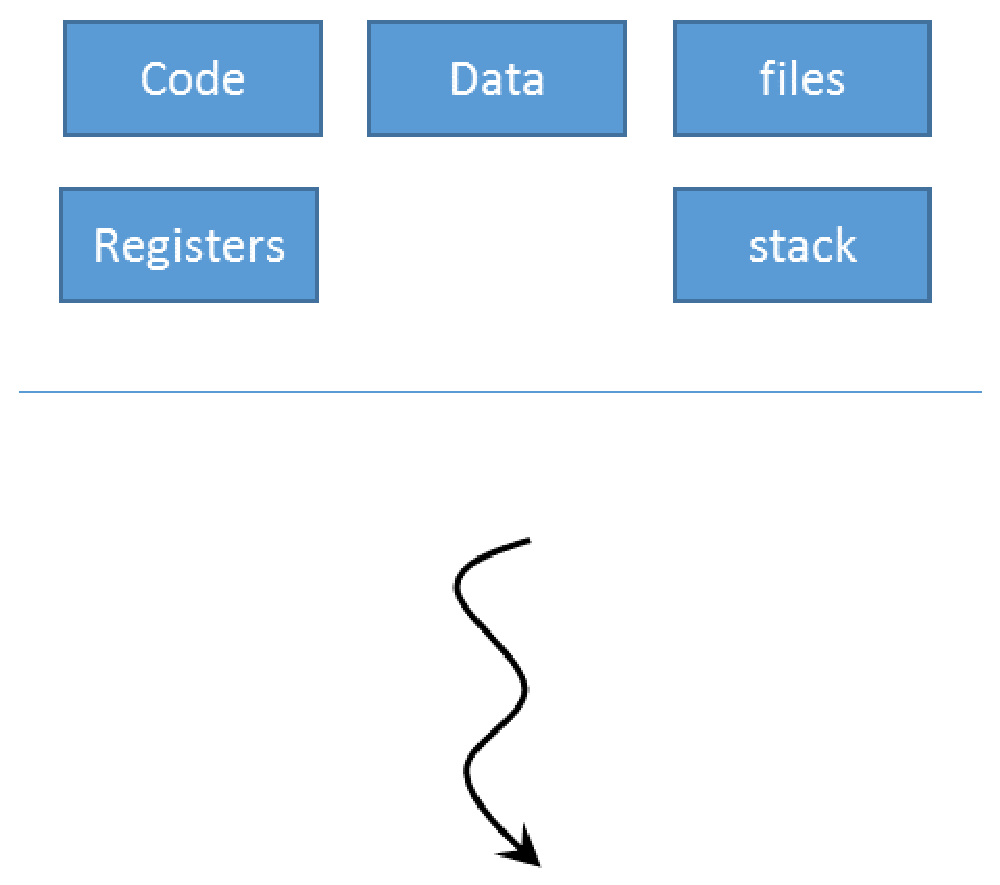
\includegraphics[scale=.25]{thread1}
	\caption{Single threaded process}
	\label{fig:thread1}
    \end{subfigure}
	\hfill
    \begin{subfigure}[b]{0.45\textwidth}
	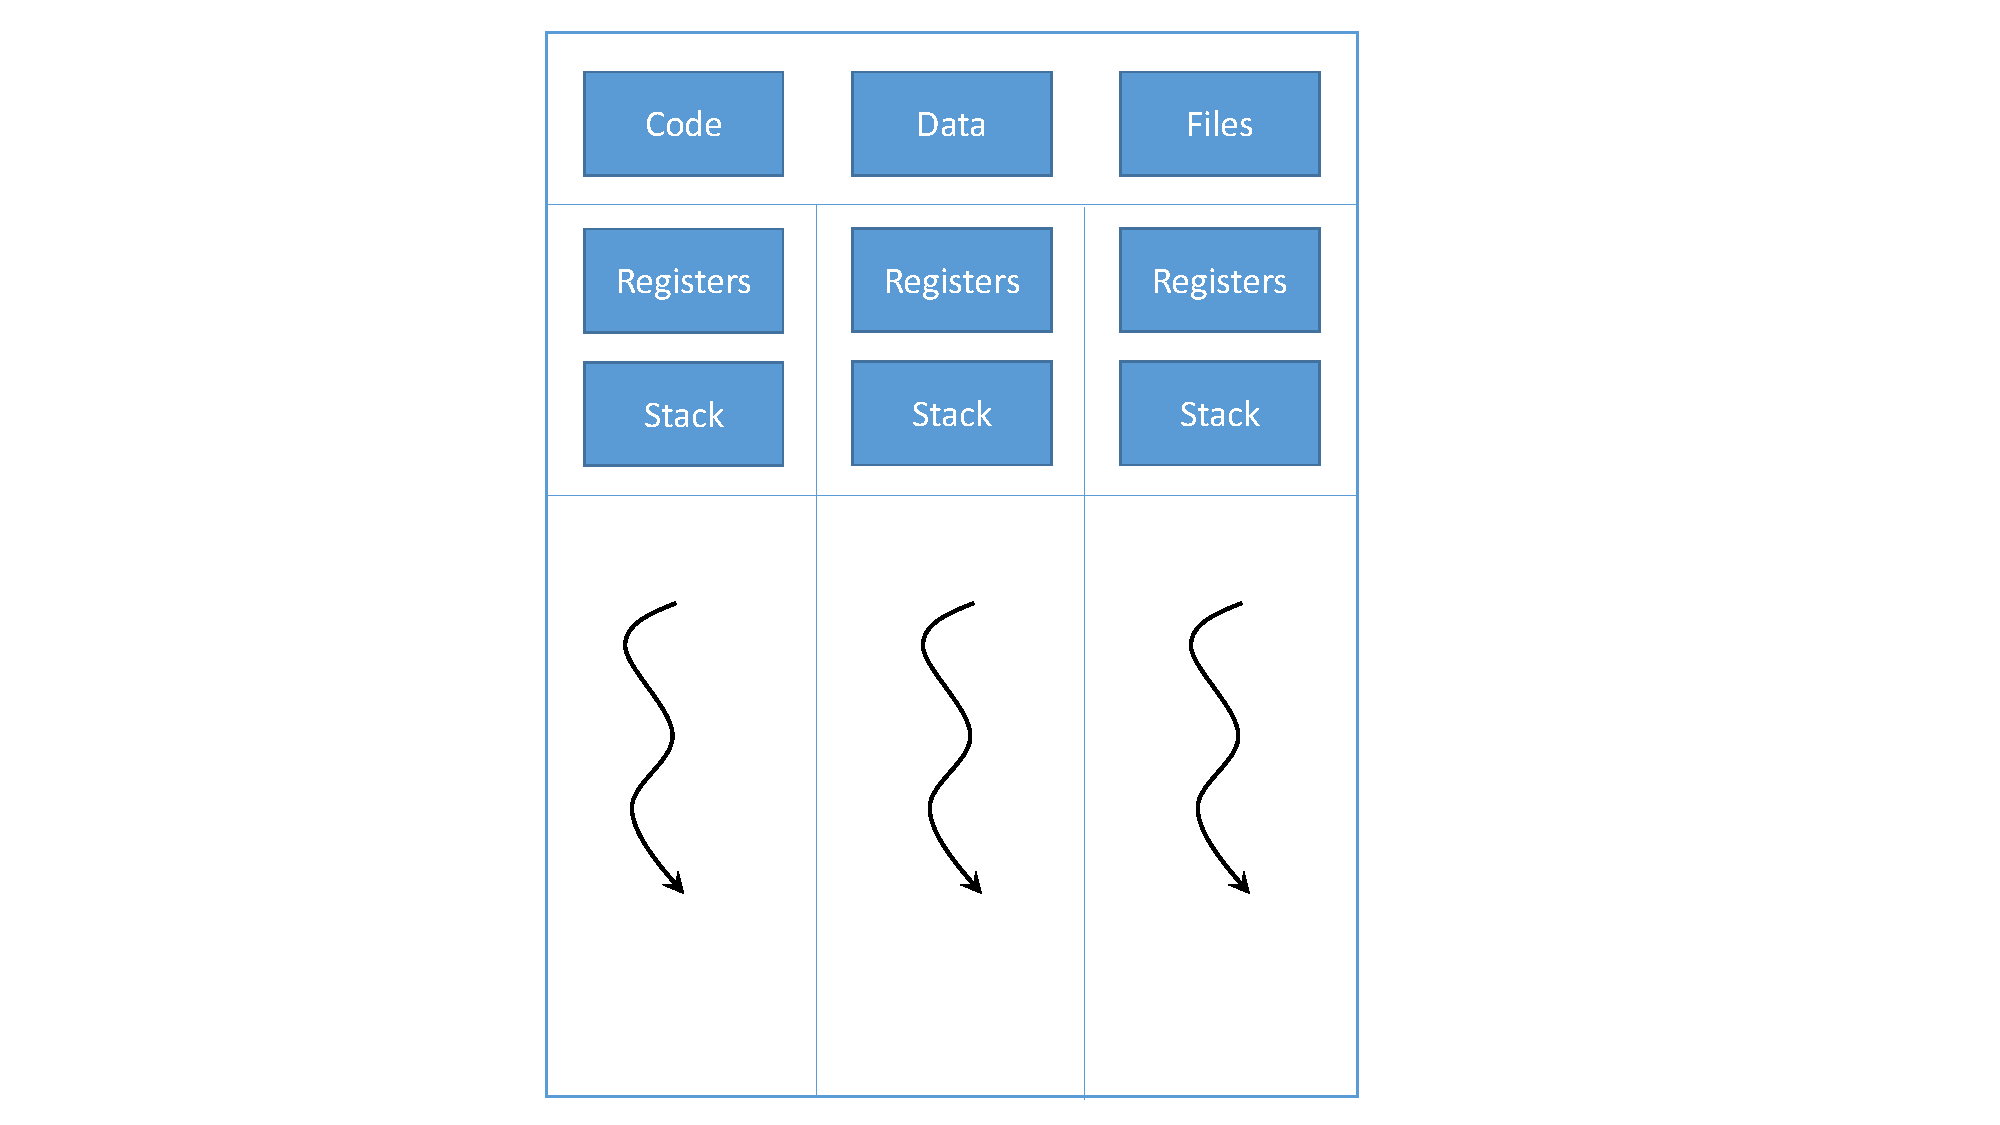
\includegraphics[scale=.25]{thread2}
	\caption{Multithreaded process}
	\label{fig:thread2}
    \end{subfigure}
    \caption{Thread}\label{fig:threads}
\end{figure}

\section{Context Switch}
Multithreading is implemented by time division multiplexing on a single processor. In time division multiplexing, the processor switches between different threads. The switch between threads is called the context switch. The context switch makes the user feel that the threads or tasks are running concurrently. However, on a multi-processor system, threads can run truly concurrently, with every processor executing a separate thread simultaneously. 
\\
In a context switch the state of a process is stored and restored, so that the execution can be resumed from the same point at a later time. The state of the process is also called a context. The context is determined by the processor and the operating system. Context switching makes it possible for multiple processes or threads to share a single processor. Usually context switches are computationally intensive. Switching between two process requires good amount of computation and time, by saving and loading registers, maping the memory, and updating various tables~\cite{Galvin} .

\section{Spinlocks}
Spinlock is one of the locking mechanisms designed to work in a multi-processing environment. Spinlock causes a thread that is trying to acquire the lock to spin in case of unavailability of it. Spinlocks are similar to the semaphores, except that when a process finds the lock closed by another process, it spins around continuously until it obtains the lock. Spinning is implemented by executing an instruction in a loop~\cite{Bovet:2005:ULK:1077084}.
\\[3mm]
In a uniprocessor environment, the waiting process keeps spinning for the lock. As the other process holding the lock might not have a chance to release it, the spinlock could deteriorate the performance in a uniprocessor environment. Howerver, in a multi-processor environment spinlocks can be more efficient. 
\\[3mm] 
In uniprocessor and multiprocessor environment, a context switch takes a significant amount of time. In a multi-processor environment, it is more efficient for each process to keep its own CPU and spin while waiting for the resource~\cite{Bovet:2005:ULK:1077084}. As a spinlock avoids the overhead of re-scheduling and context switching, spinning for a short time can be more efficient than a context switch. For the same reason, spinlocks are often used inside operating system kernels.
\\[3mm]
\textbf{Adaptive Spinning} is a spinlock optimization technique. In the adaptive spinning technique, the duration of the spin is determined by policy decisions based on the rate of success and failure of recent spin attempts on the same lock. Adaptive spinning helps threads to avoid spinning in futile conditions.

\section{Device Driver}
\label{sec:device driver}
A device driver is a program that provides a software interface to a particular hardware device. It enables the operating system and other programs to access the hardware functions. Device drivers are hardware dependent and operating system specific. When a program invokes a routine in the driver, the driver issues commands to the device. After execution, the device sends data back to the driver. The driver may invoke routines in the original calling program after recieving the data. The Linux distinguishes between three fundamental device types: character device, block device and network interface. Each kernel module usually implements one of these types.
\begin{figure}[!ht]
\centering
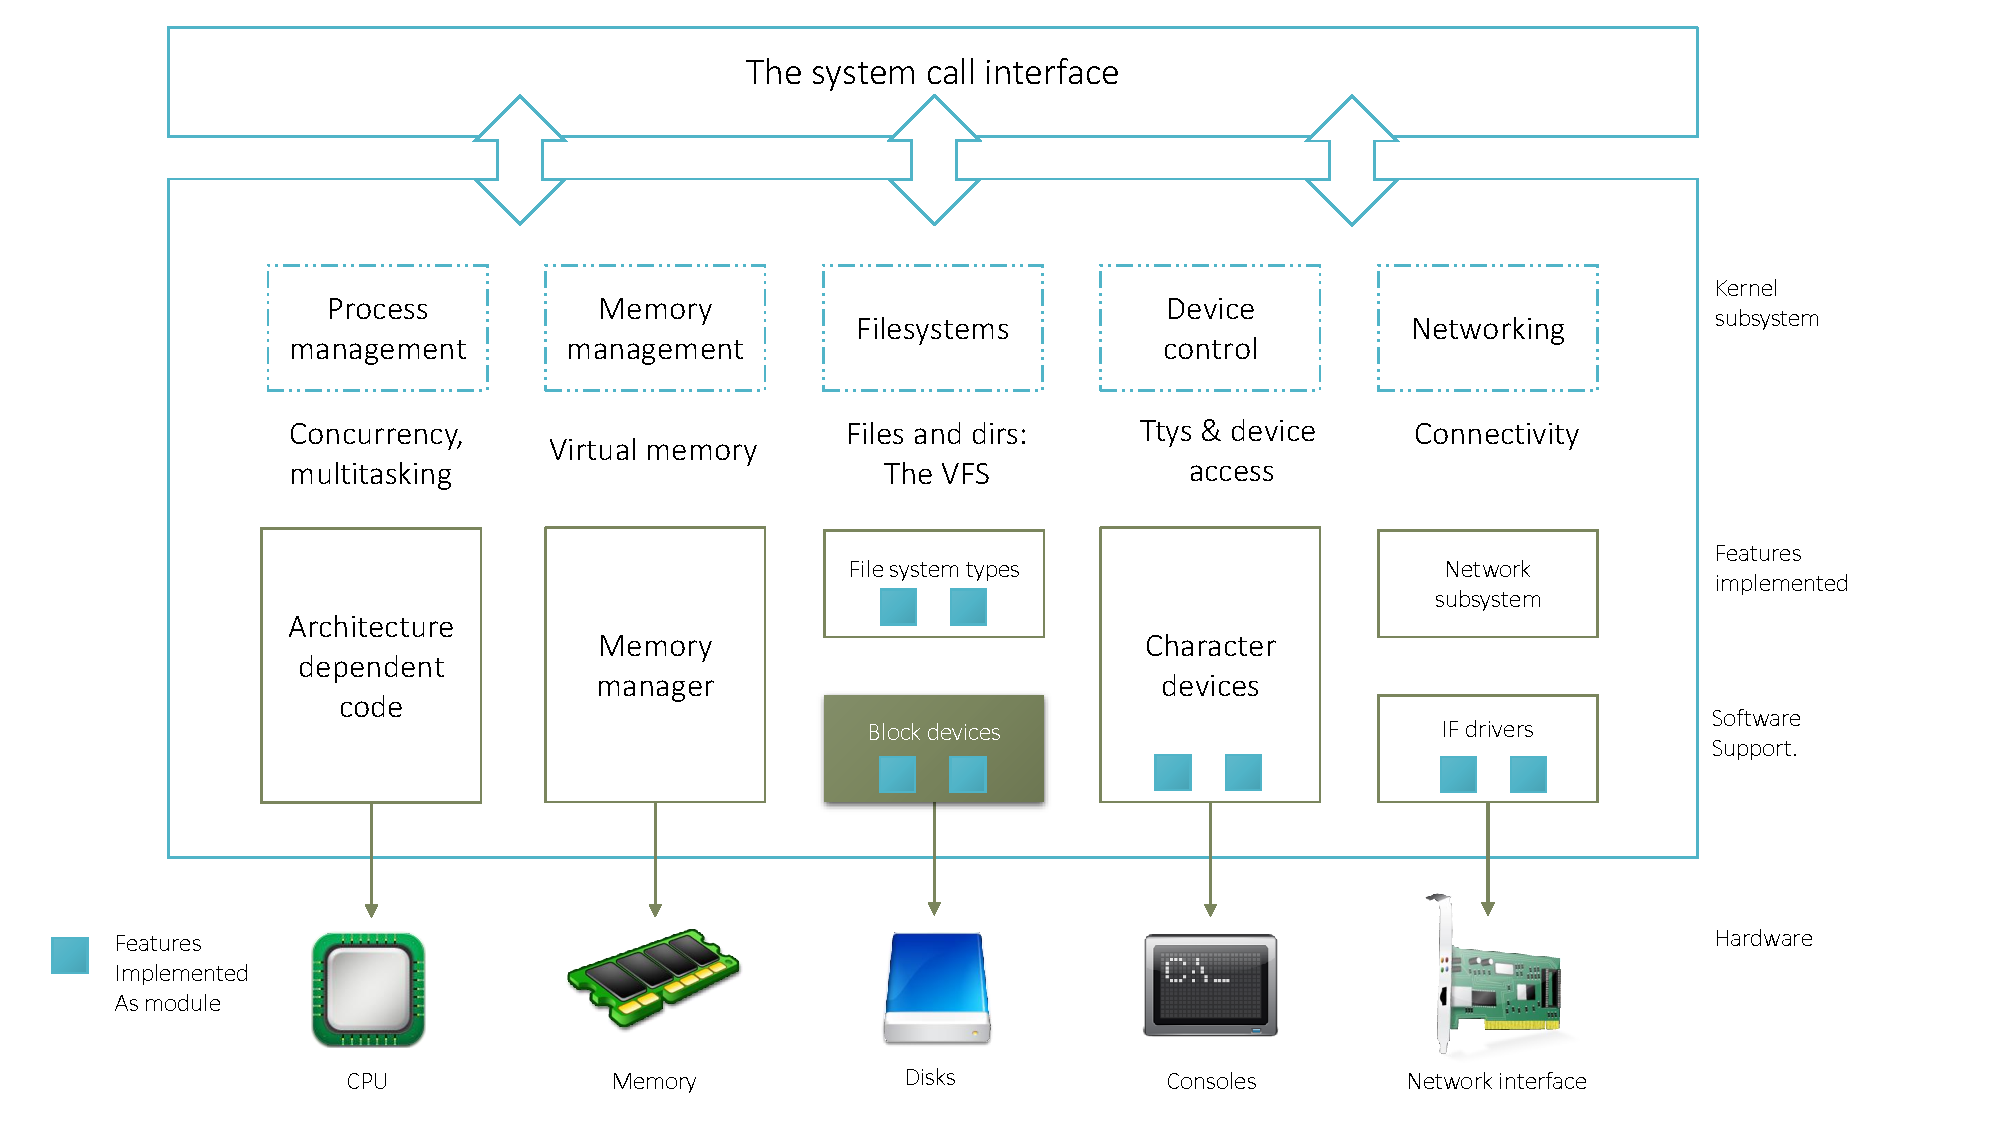
\includegraphics[scale=.5 ]{kernel}
\caption{Split view of a kernel}
\label{fig:kernel}
\end{figure}
\paragraph{Character devices:} A character device can be accessed as a stream of bytes. A character driver implements this behavior of the character device. A character driver usually implements at least the open, close, read, and write system calls. The text console (/dev/console) and the serial ports (/dev/ttyS0) are examples of character devices.

\paragraph{Network Interfaces:} A network interface is a device that is able to exchange data with other hosts. Usually, a network interface is a hardware device, but it can be a software device like the loopback interface. 

\paragraph{Block Devices:} A block device is a device that can host a filesystem. Block devices are accessed by filesystem nodes in the /dev directory. In most unix implementations, a block device can only handle I/O operations that transfer one or more whole blocks. Linux, instead, allows the application to read and write any number of bytes on a block device. As a result, block and char devices differ only in the way data is managed internally by the kernel, and thus block drivers have a completely different interface than char drivers. Examples of block devices are disks and CDs~\cite{Corbet:2005:LDD:1209083}.

\subsection*{Block Device Driver}
\subsubsection*{Request processing in a block device driver}
\label{subsec:request queue}
The core of every block driver is its request function. The request function is called whenever the driver needs to process reads, writes, or other operations on the device. The request function does not need to actually complete all of the requests on the queue before it returns. However, it ensures that all the requests are eventually processed by the driver. The block device driver request method accepts a parameter which acts as a pointer to the request queue. Every device has a separate request queue. A spinlock is needed as part of the request queue creation process. A request function of the device is associated with the request queue in its creation process. The kernel holds the spinlock whenever the request function is called. As a result, the request function runs in an atomic context.
\\[3mm]
Each request structure represents one block I/O request, however, it might be formed through a merger of several independent requests at a higher level.
The kernel may join multiple requests that involve adjacent sectors on the disk, but it never combines read and write operations within a single request structure. A request structure is implemented as a linked list of bio structures. The bio structure is a low-level description of a portion of a block I/O request~\cite{Corbet:2005:LDD:1209083}.

\subsubsection*{The bio structure}
The kernel describes a read or write operation of a block device in the form of a bio structure. The bio structure has a everything that a block device driver needs to execute the request, without reffering to the user space process that caused the request to be initiated. After creation, the bio structure is handed to the block I/O code. The block I/O code merges the bio structure into an existing request structure, otherwise it creates a new request~\cite{Corbet:2005:LDD:1209083}. 

\section{Memory Protection}
The memory protection mechanism of a computer system controls the access to objects. The main goal of memory protection is to prevent malicious misuse of the system by users or programs. Memory protection also ensures that each shared resource is used only in accordance with the system policies. In addition, it also helps to ensure that errant programs cause minimal damage. However, memory protection systems only provide the mechanisms for enforcing policies and ensuring reliable systems. It is up to the administrators, programmers and users to implement those mechanisms~\cite{Galvin, Graham:1971:PPP:1478873.1478928}. Subsection~\ref{subsec:user level} and subsection~\ref{subsec:kernel level} explain the policies implemented at kernel level and user level. 

\subsection{User Level}
\label{subsec:user level}
Typically in a monolithic kernel, the lowest \texttt{X Gb} of memory is reserved for user processes. The upper \texttt{Virtual Memory size - X Gb} is reserved for the kernel. This upper \texttt{VM-X Gb} is restricted to \texttt{CPL 0} only. The kernel puts its private data structures in the upper memory and always accesses them at the same virtual address. 
\begin{figure}[!ht]
\centering
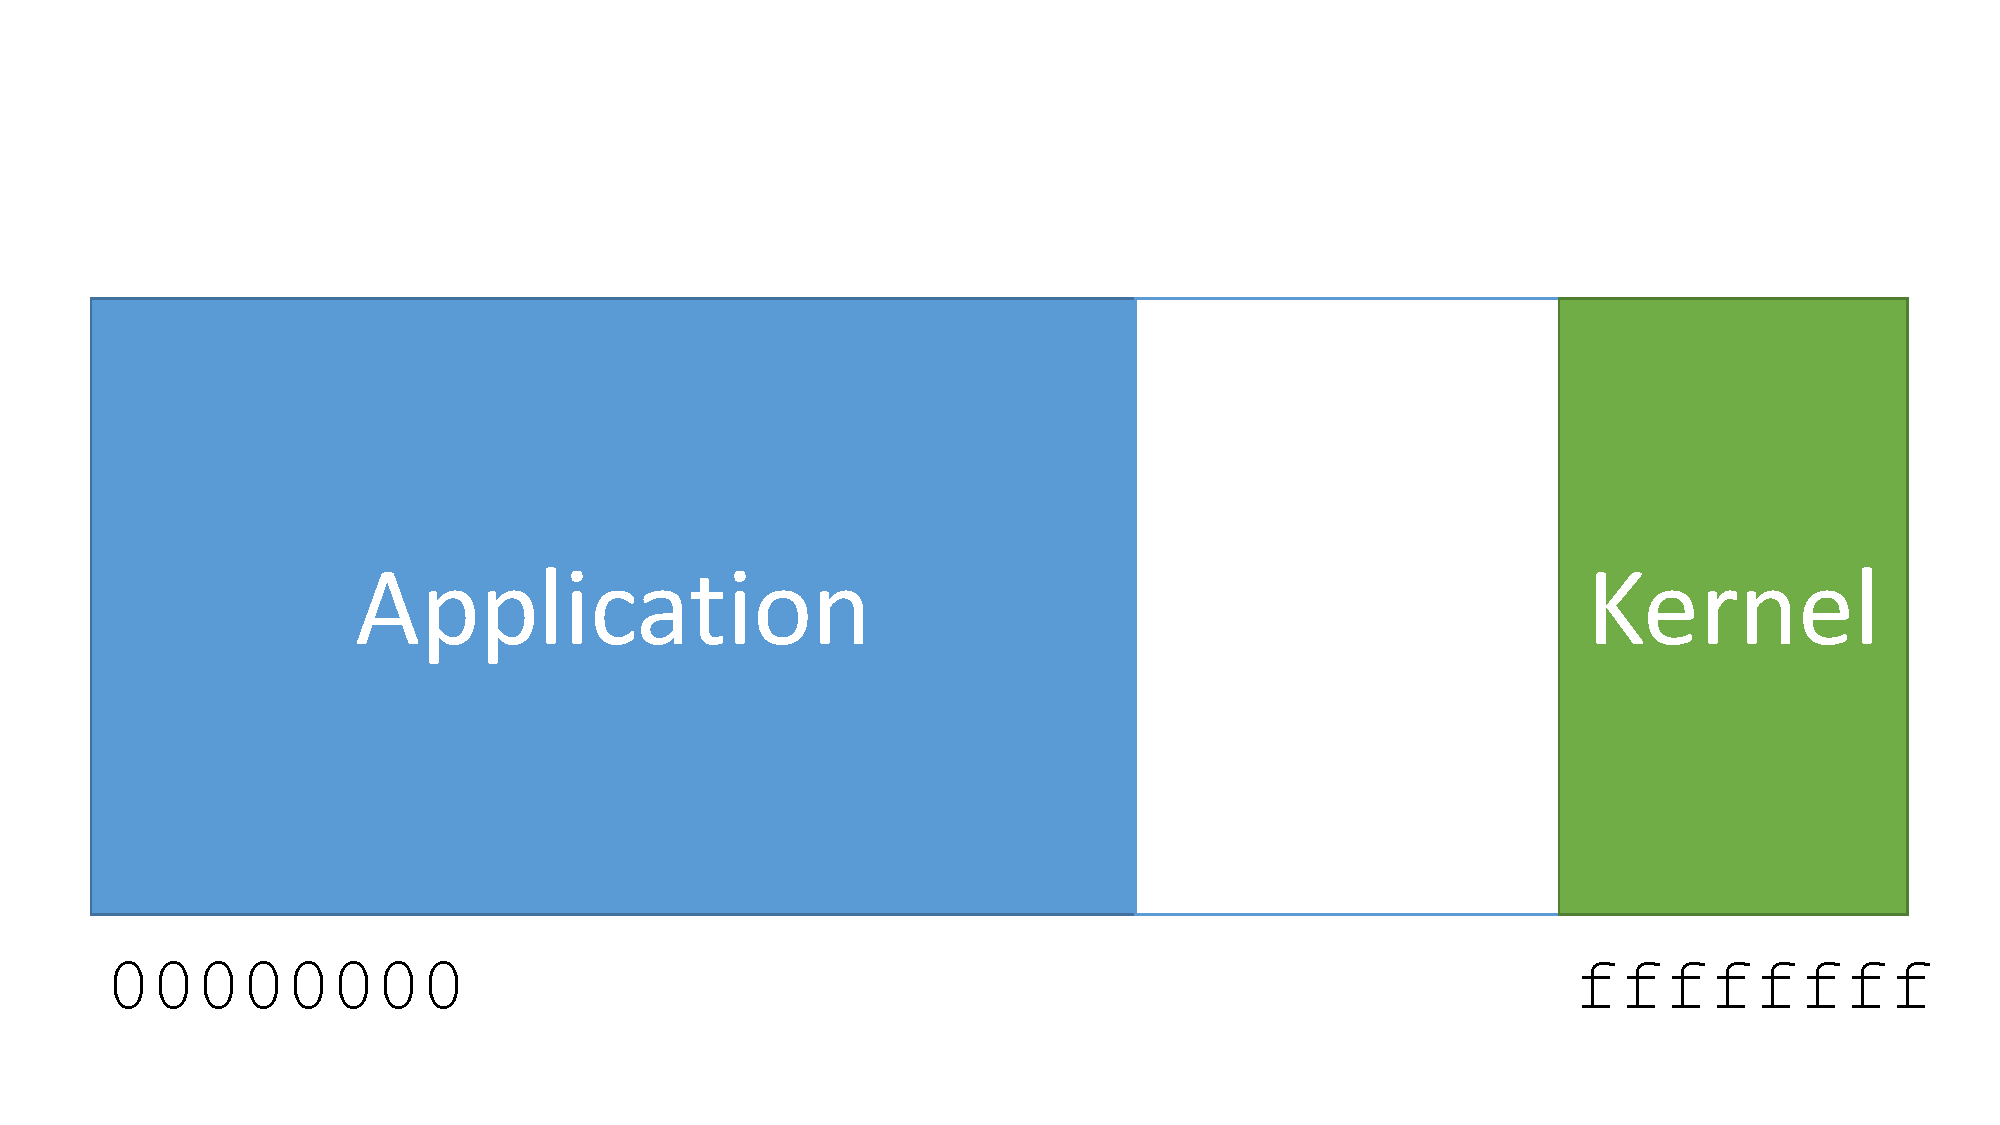
\includegraphics[scale=.25 ]{memory_map}
\caption{Physical memory}
\label{fig:memmap}
\end{figure}
\\[3mm]
At the user space, each application runs as a separate process. Each process is associated with an address space and believes that it owns the entire memory, starting with the virtual address 0. However, a translation table translates every memory reference by these processes from virtual to physical addresses. The translation table maintains \texttt{$<$base, bound$>$} entry. If a process tries to access virtual address that is outside the \texttt{base + bound} address, then an error is reported by the operating system, otherwise the physical address \texttt{base + virtual address} is returned. This allows multiple processes to be run in the memory with protection. Since address translation provides protection, a process canot access the address outside its address space.
\\[3mm]
Consider an example in Figure~\ref{fig:User space}.
\begin{enumerate}
\item The system is running 3 different processes in a user space.
\item One of the processes hits a bug and tries to corrupt the memory outside the address space.
\item Access to the address is restricted by the memory protection mechanism.
\begin{figure}[!ht]
    \centering
    \begin{subfigure}[b]{0.49\textwidth}
	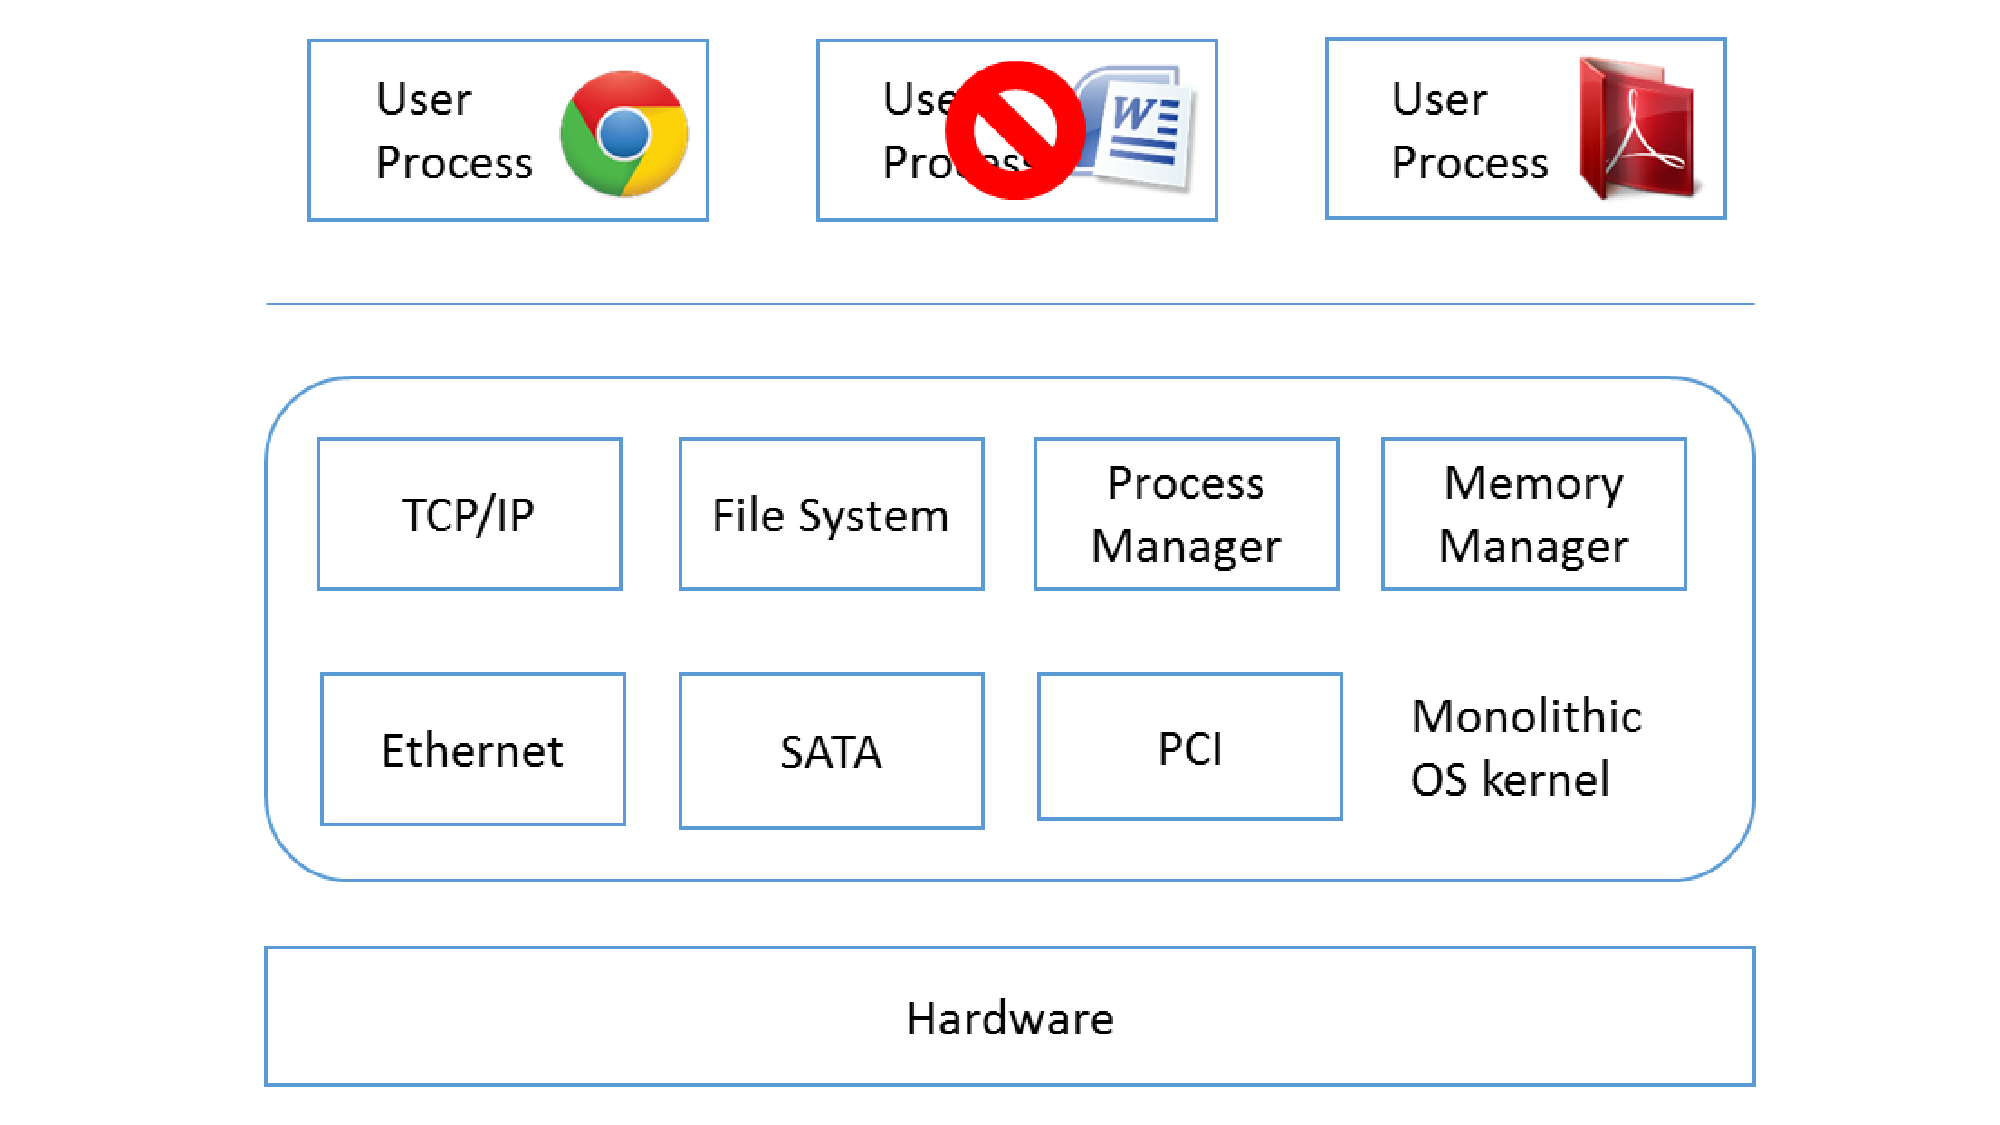
\includegraphics[scale=.25]{user-space-1}
	\caption{A process hits a bug}
    \end{subfigure}
	\hfill
    \begin{subfigure}[b]{0.49\textwidth}
	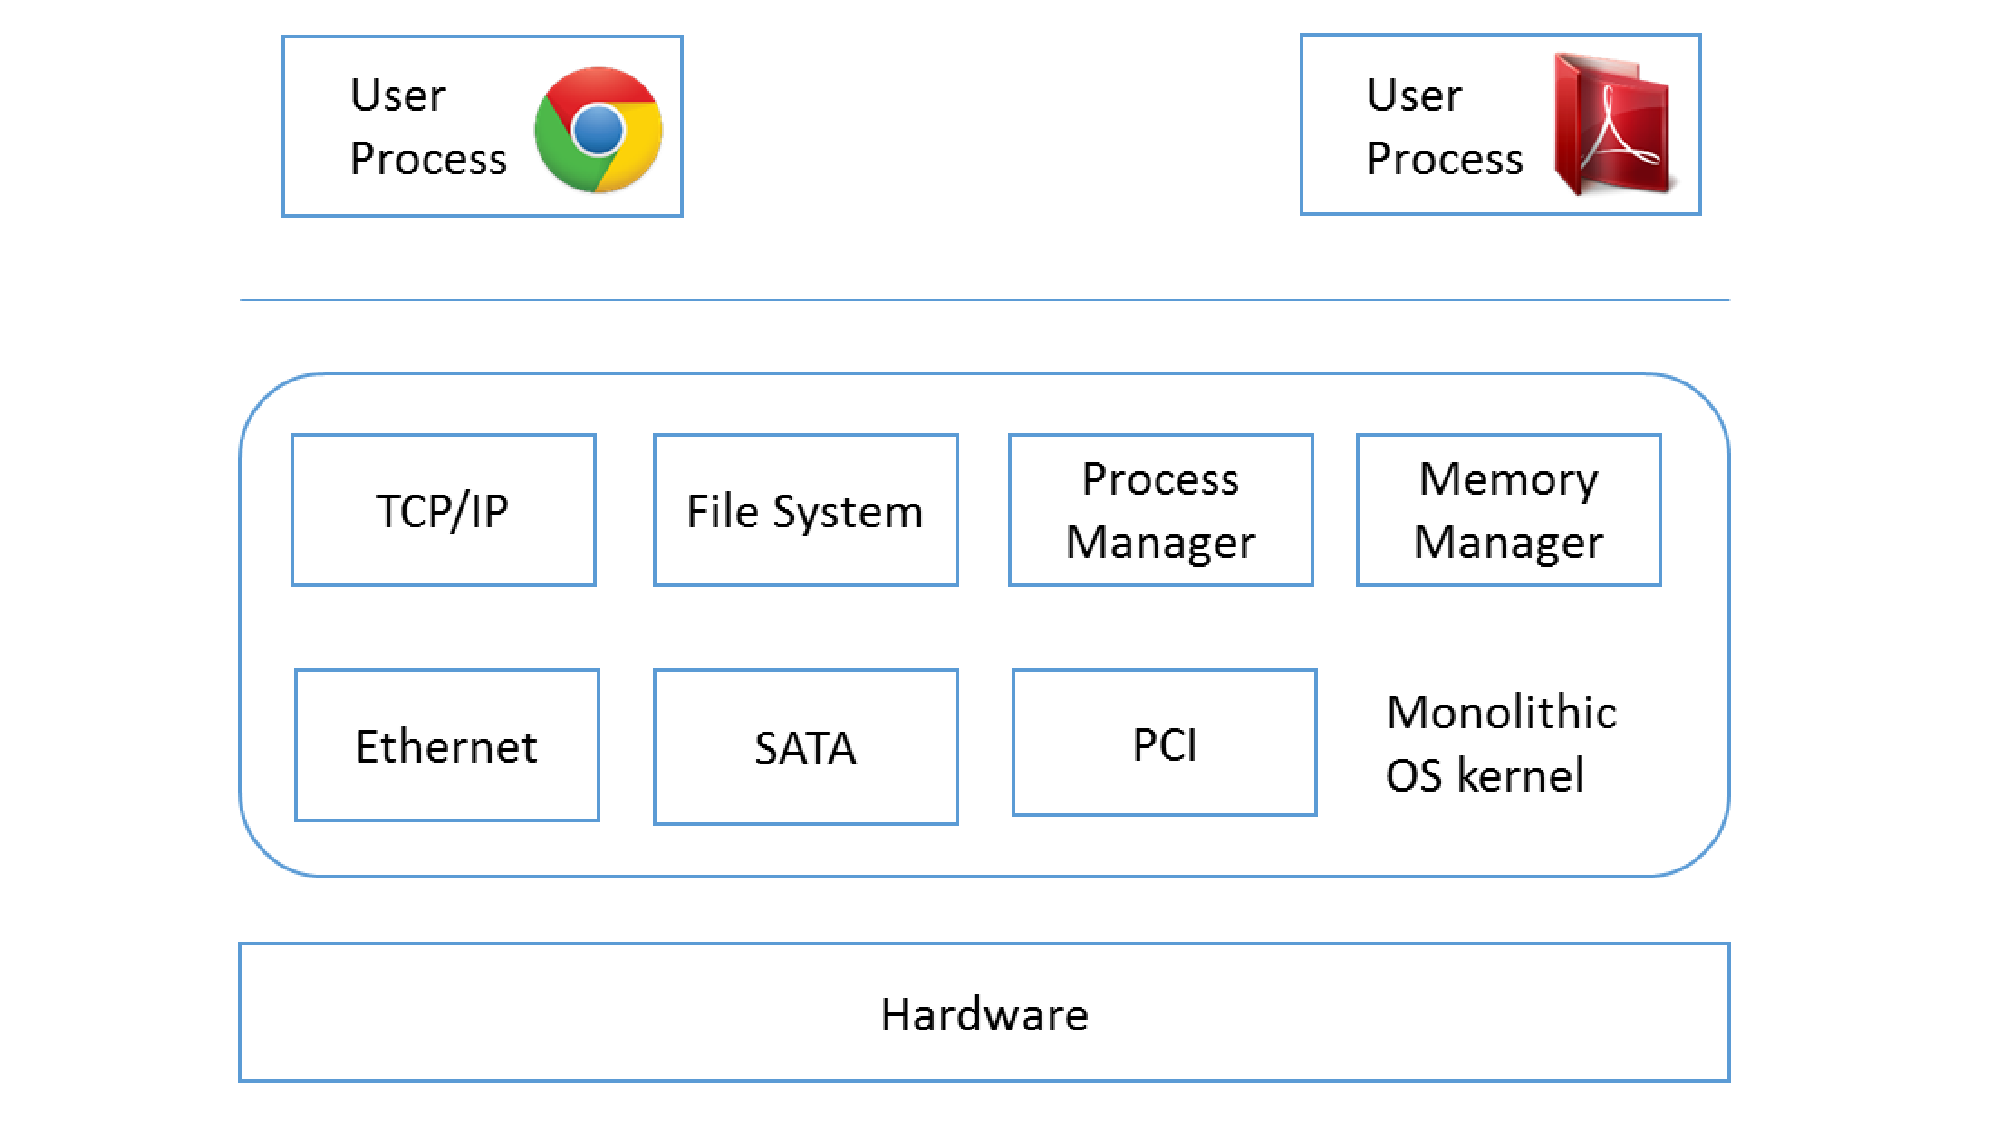
\includegraphics[scale=.25]{user-space-2}
	\caption{Intact system}
    \end{subfigure}
    \caption{User level memory protection}\label{fig:User space}
\end{figure}
\end{enumerate}

\subsection{Kernel Level}
\label{subsec:kernel level}
Kernel reserves upper \texttt{Virtual memory size - X Gb} of virtual memory for its internal use. The page table entries of this region are marked as protected so that pages are not visible or modifiable in the user mode. This reserved region is divided into two regions. First region contains page table references to every page in the system. It is used to do translations of addresses from physical to virtual when the kernel code is executed. The core of the kernel and all the pages allocated by page allocator lies in this region. The other region of the kernel memory is used by the memory allocator, the allocated memory is mapped by kernel modules. Since an operating system maps physical addresses directly, kernel components do not have memory protection similar to that of the user space. At kernel level any code running at \texttt{CPL 0} can access the kernel memory, hence a kernel component can access, and potentially, corrupt the kernel data structures. 
\\[3mm]
Consider an example shown in the Figure~\ref{fig:Kernel space}.
\begin{enumerate}
\item The system runs 3 different processes in the user space and has different kernel components running in the kernel space.
\item The network driver hits a bug, and corrupts the kernel data structure. The corruption might lead to a system crash.
\end{enumerate}
\begin{figure}[!ht]
    \centering
    \begin{subfigure}[b]{0.49\textwidth}
	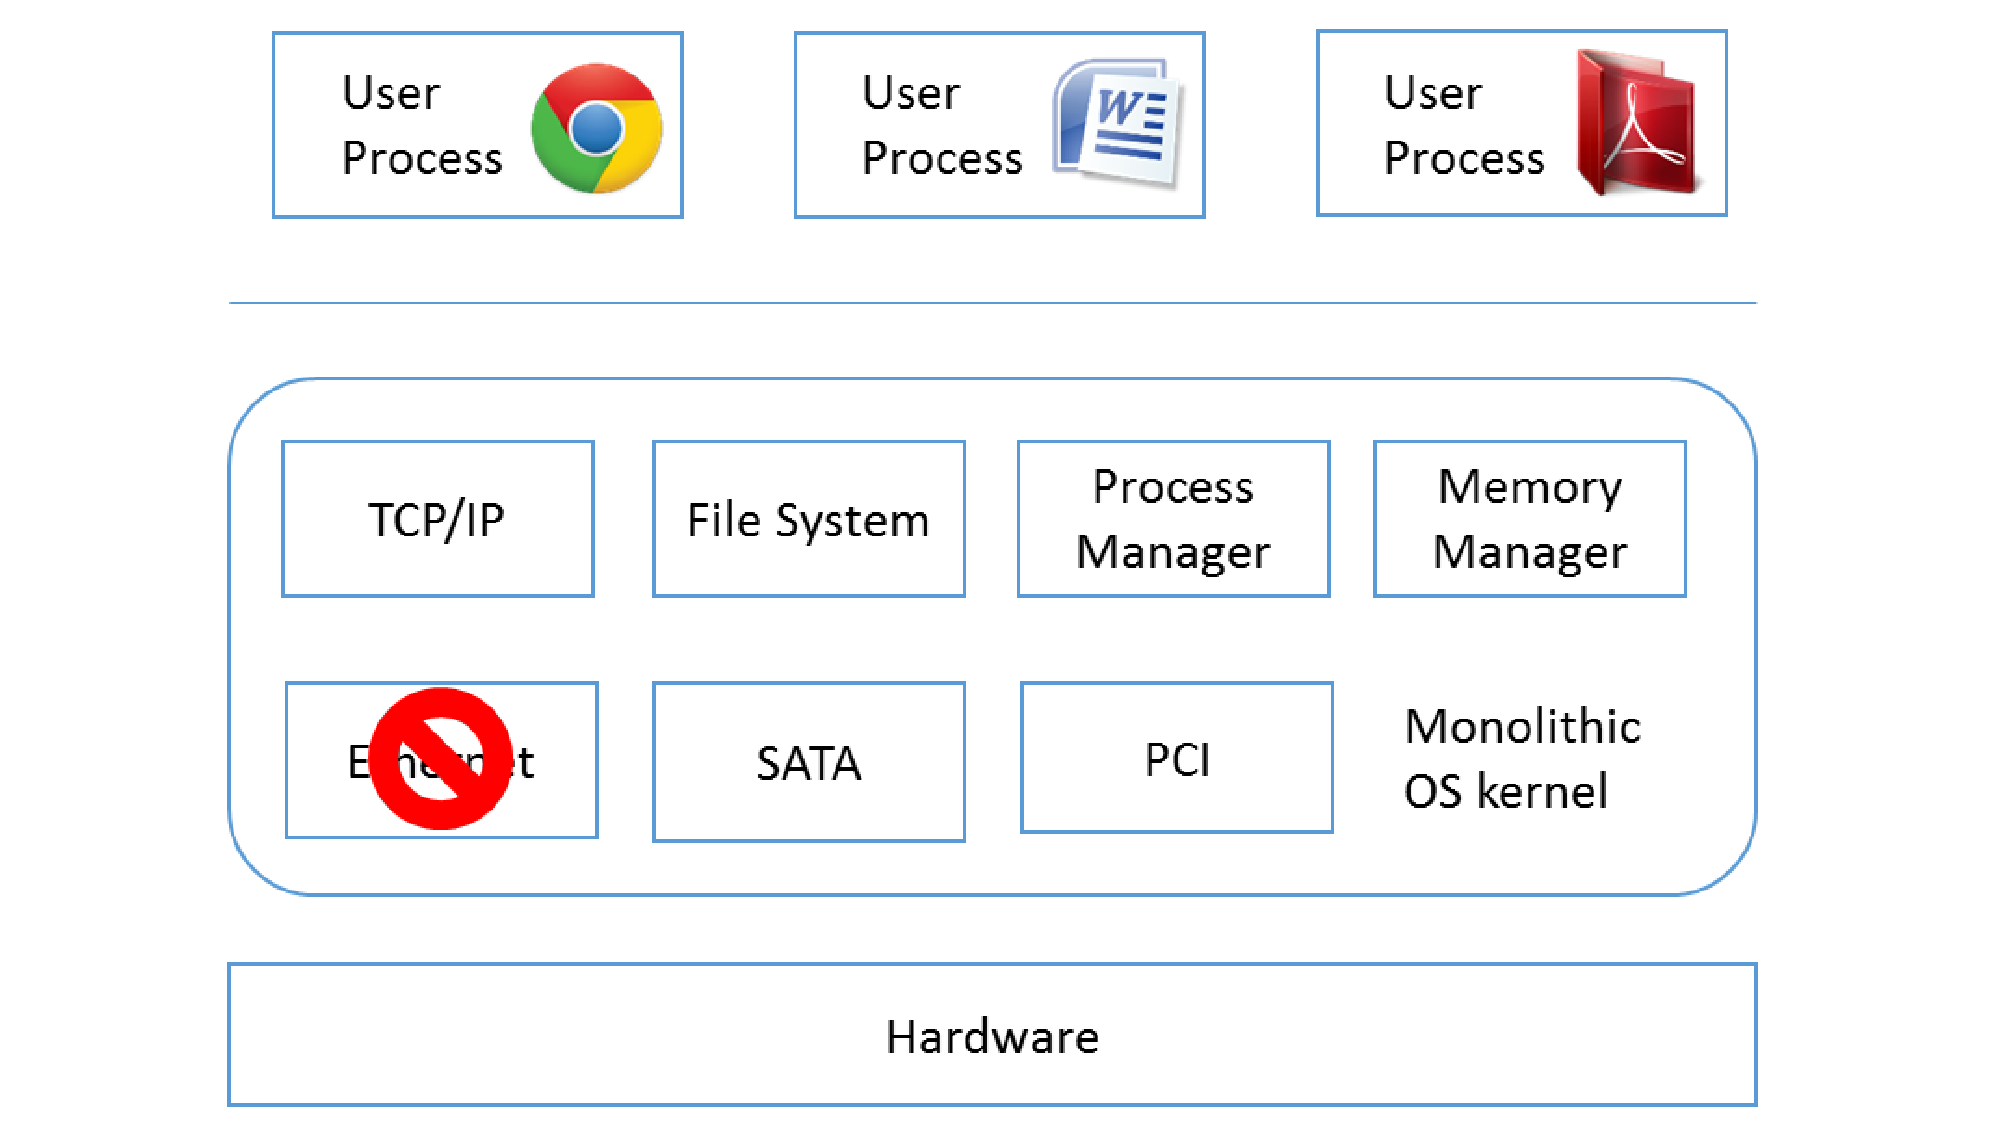
\includegraphics[scale=.25]{kernel-space-1}
	\caption{A kernel component hits a bug}
    \end{subfigure}
	\hfill
    \begin{subfigure}[b]{0.49\textwidth}
	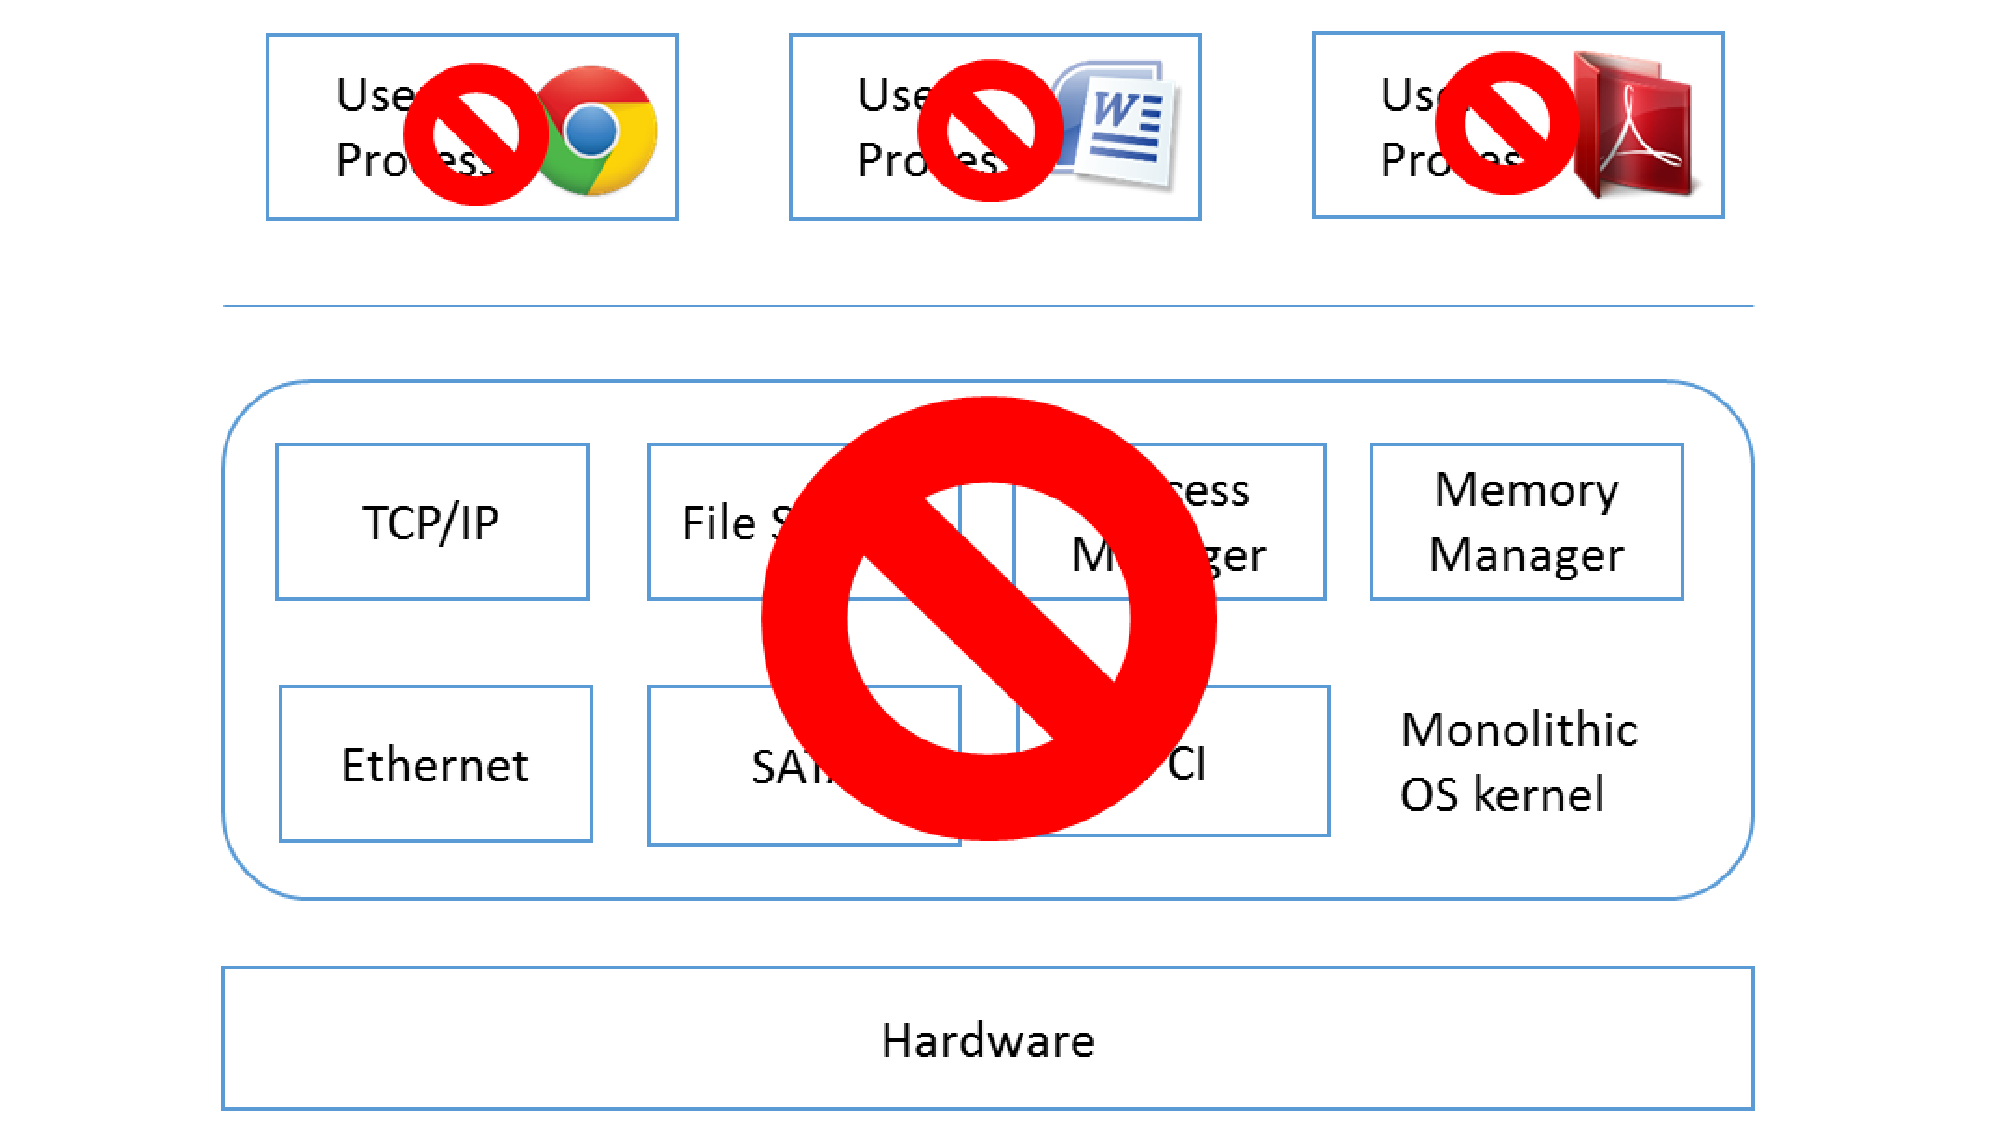
\includegraphics[scale=.25]{kernel-space-2}
	\caption{Results in a system crash}
    \end{subfigure}
    \caption{Kernel level memory protection}\label{fig:Kernel space}
\end{figure}

\section{Virtualization}
Virtualization is the act of creating a virtual version of a hardware platform, storage device, or computer network resource etc. In an operating system virtualization, the software allows a hardware to run multiple operating system images at the same time.
\\[3mm]
Virtualization has the capability to share the underlying hardware resources and still provide an isolated environment to each operating system. In virtualization, each operating system runs independently from the other on its own virtual processors. Because of this isolation the failures in an operating system are contained. Virtualization is implemented in many different ways. It can be implemented either with or without hardware support. Also operating systems might require some changes in order to run in a virtualized environment~\cite{Drepper:2008:CV:1348583.1348591}. It has been shown that virtualization can be utilized to provide better security and robustness for operating systems~\cite{Fraser04safehardware, LeVasseur04UnmodifiedDriverReuse, Riley:2008:GPK:1433006.1433008}.
\begin{figure}[!ht]
    \centering
    \begin{subfigure}[b]{0.49\textwidth}
	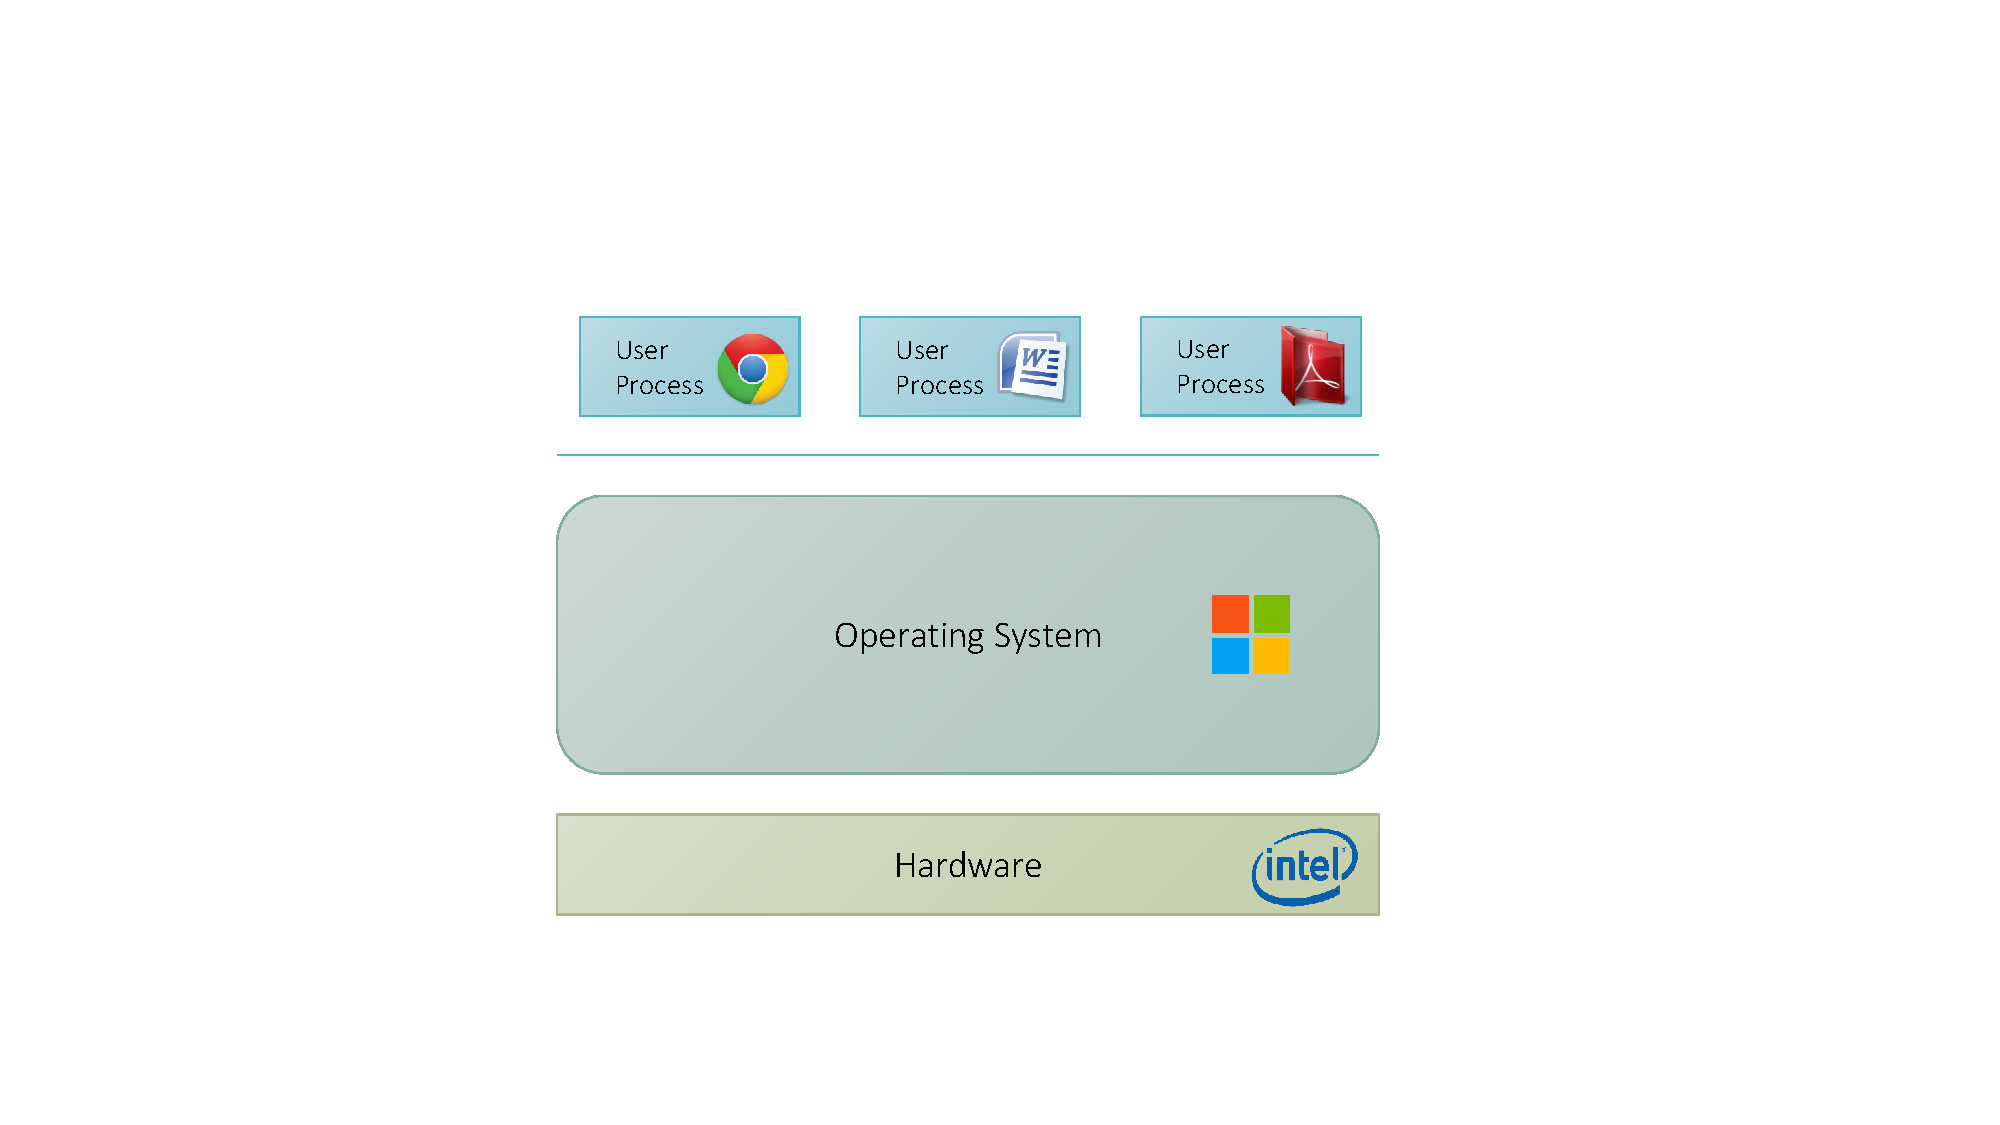
\includegraphics[scale=.25]{OS-arch}
	\caption{Operating System Architecture}
	\label{fig:OS}
    \end{subfigure}
	\hfill
    \begin{subfigure}[b]{0.49\textwidth}
	\includegraphics[scale=.25]{Virtualization}
	\caption{Virtualization}
	\label{fig:Virtualization}
	\end{subfigure}
    \caption{Comparision of a non-virtualized system and a virtualized system}\label{fig:Kernel space}
\end{figure}

\subsection{Hypervisor}
Hypervisor is a piece of computer software, firmware or hardware that creates and runs virtual machines. Operating system virtualization is achieved by inserting a hypervisor between the guest operating system and the underlying hardware. Most of the literature presents hypervisor synonymous to a virtual machine monitor (VMM). While, VMM is a software layer specifically responsible for virtualizing a given architecture, a hypervisor is an operating system with a VMM. The operating system may be a general purpose one, such as Linux, or it may be developed specifically for the purpose of running virtual machines~\cite{Agesen:2010:EXV:1899928.1899930}.
\\[3mm]
A computer on which a hypervisor is running one or more virtual machines is defined as a host machine. Each virtual machine is called a guest machine. The hypervisor presents the guest operating systems with a virtual operating platform and manages the execution of the guest operating systems. Multiple instances of a variety of operating systems share the virtualized hardware resources. Among widely known hypervisors are Xen~\cite{Barham:2003:XAV:1165389.945462, Chisnall:2007:DGX:1407351}, KVM~\cite{Habib:2008:VK:1344209.1344217, kivity07kvm}, VMware ESX~\cite{Agesen:2010:EXV:1899928.1899930} and VirtualBox~\cite{citeulike:3149886}.
\\[3mm]
There are two types of hypervisors~\cite{Goldberg:1973:AVM:800122.803950}
\begin{itemize}
\item Type 1 hypervisors are also called native hypervisors or bare metal hypervisors. Type 1 hypervisors run directly on the host's hardware to control the hardware and to manage guest operating systems. A guest operating-system, thus, runs on another level above the hypervisor. Type 1 hypervisors represent the classic implementation of virtual-machine architectures such as SIMMON, and CP/CMS. Modern equivalents include Oracle VM Server for SPARC, Oracle VM Server, the Xen hypervisor~\cite{Barham:2003:XAV:1165389.945462}, VMware ESX/ESXi~\cite{Agesen:2010:EXV:1899928.1899930} and Microsoft Hyper-V.
\begin{figure}[!ht]
\centering
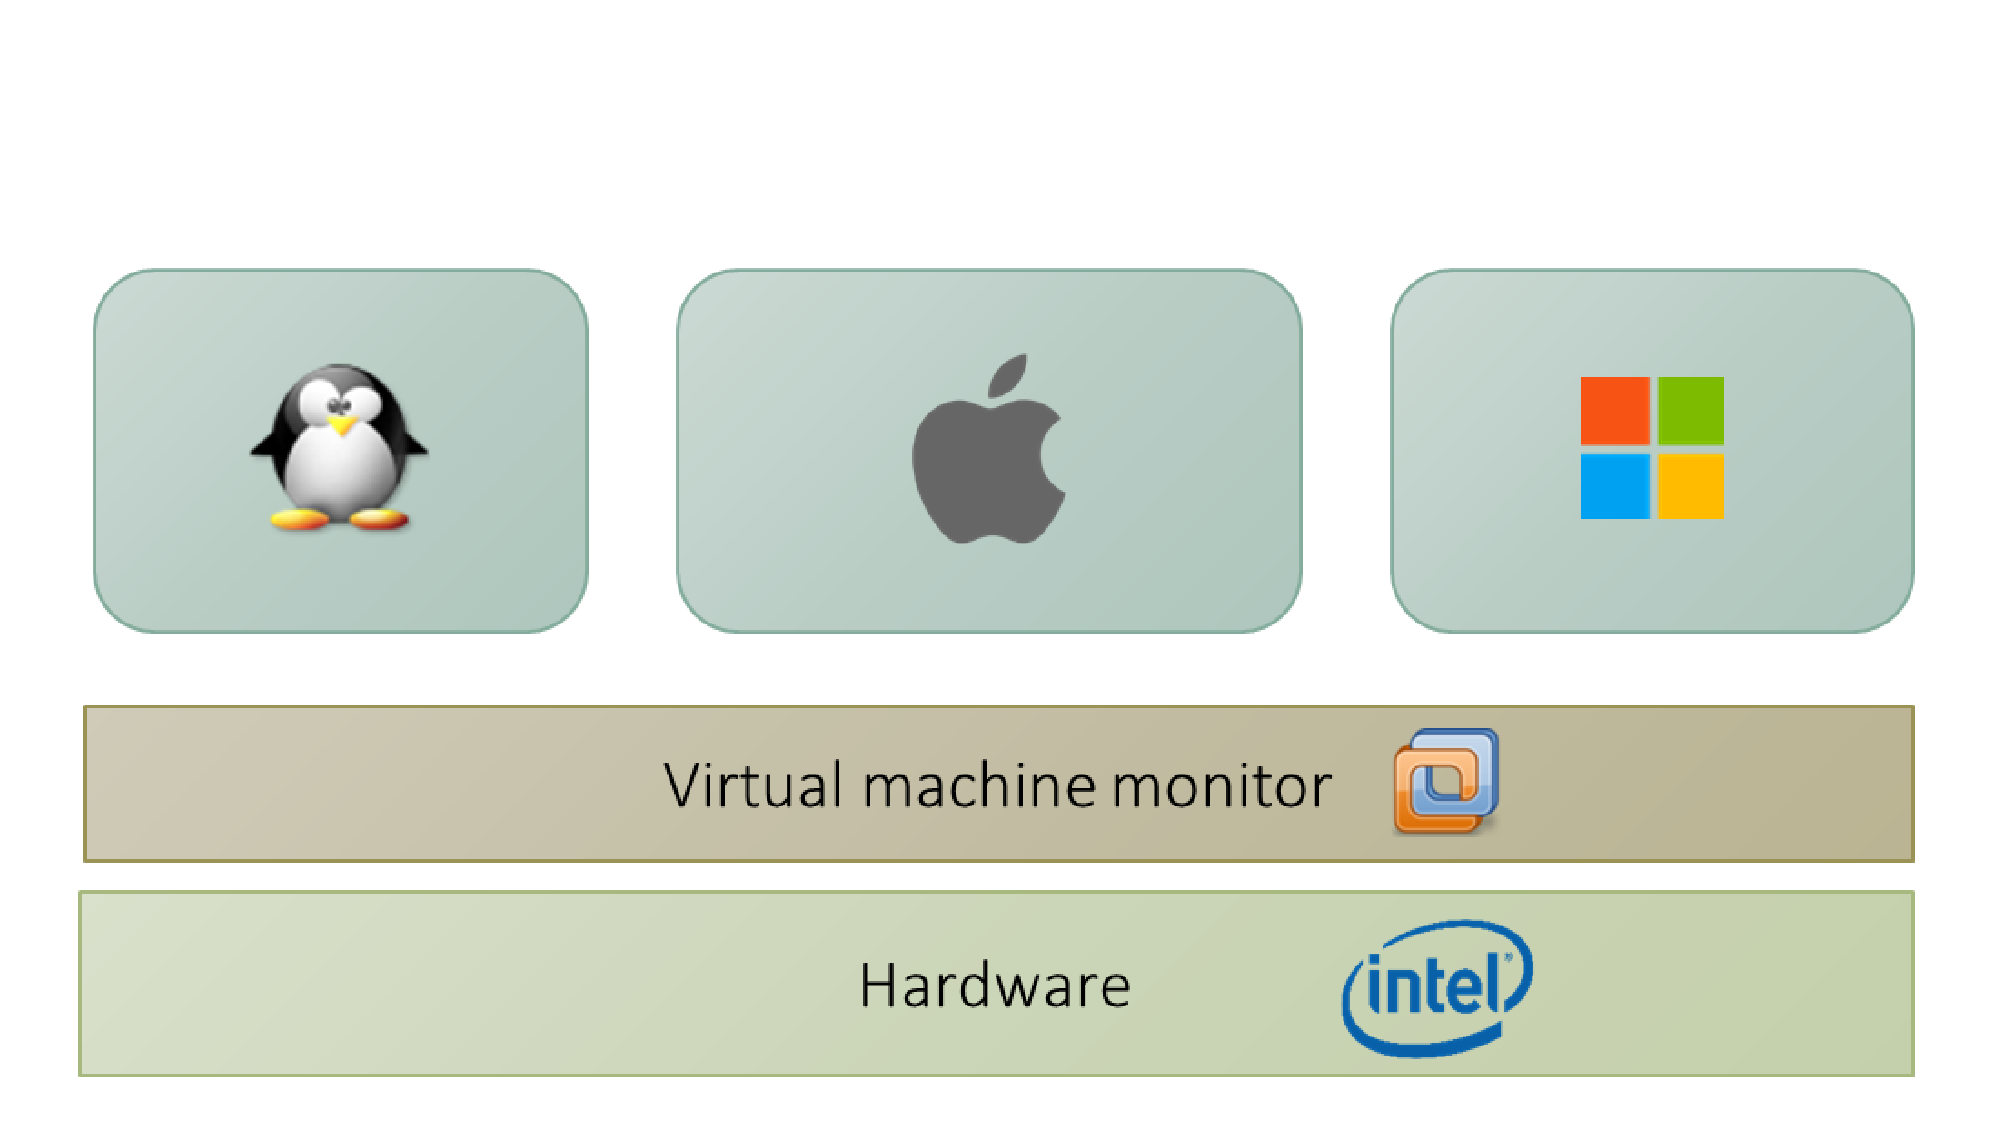
\includegraphics[scale=.35]{type1}
\caption{Type 1 hypervisor}
\label{Type 1 hypervisor}
\end{figure}
\item Type 2 hypervisors are also called hosted hypervisors. Type 2 hypervisors run within a conventional operating-system environment. Type 2 hypervisors run at a distinct second software level, whereas guest operating systems run at the third level above hardware. VMware Workstation and VirtualBox are some of the examples of Type 2 hypervisors~\cite{Sugerman:2001:VID:647055.715774, citeulike:3149886}.
\begin{figure}[!ht]
\centering
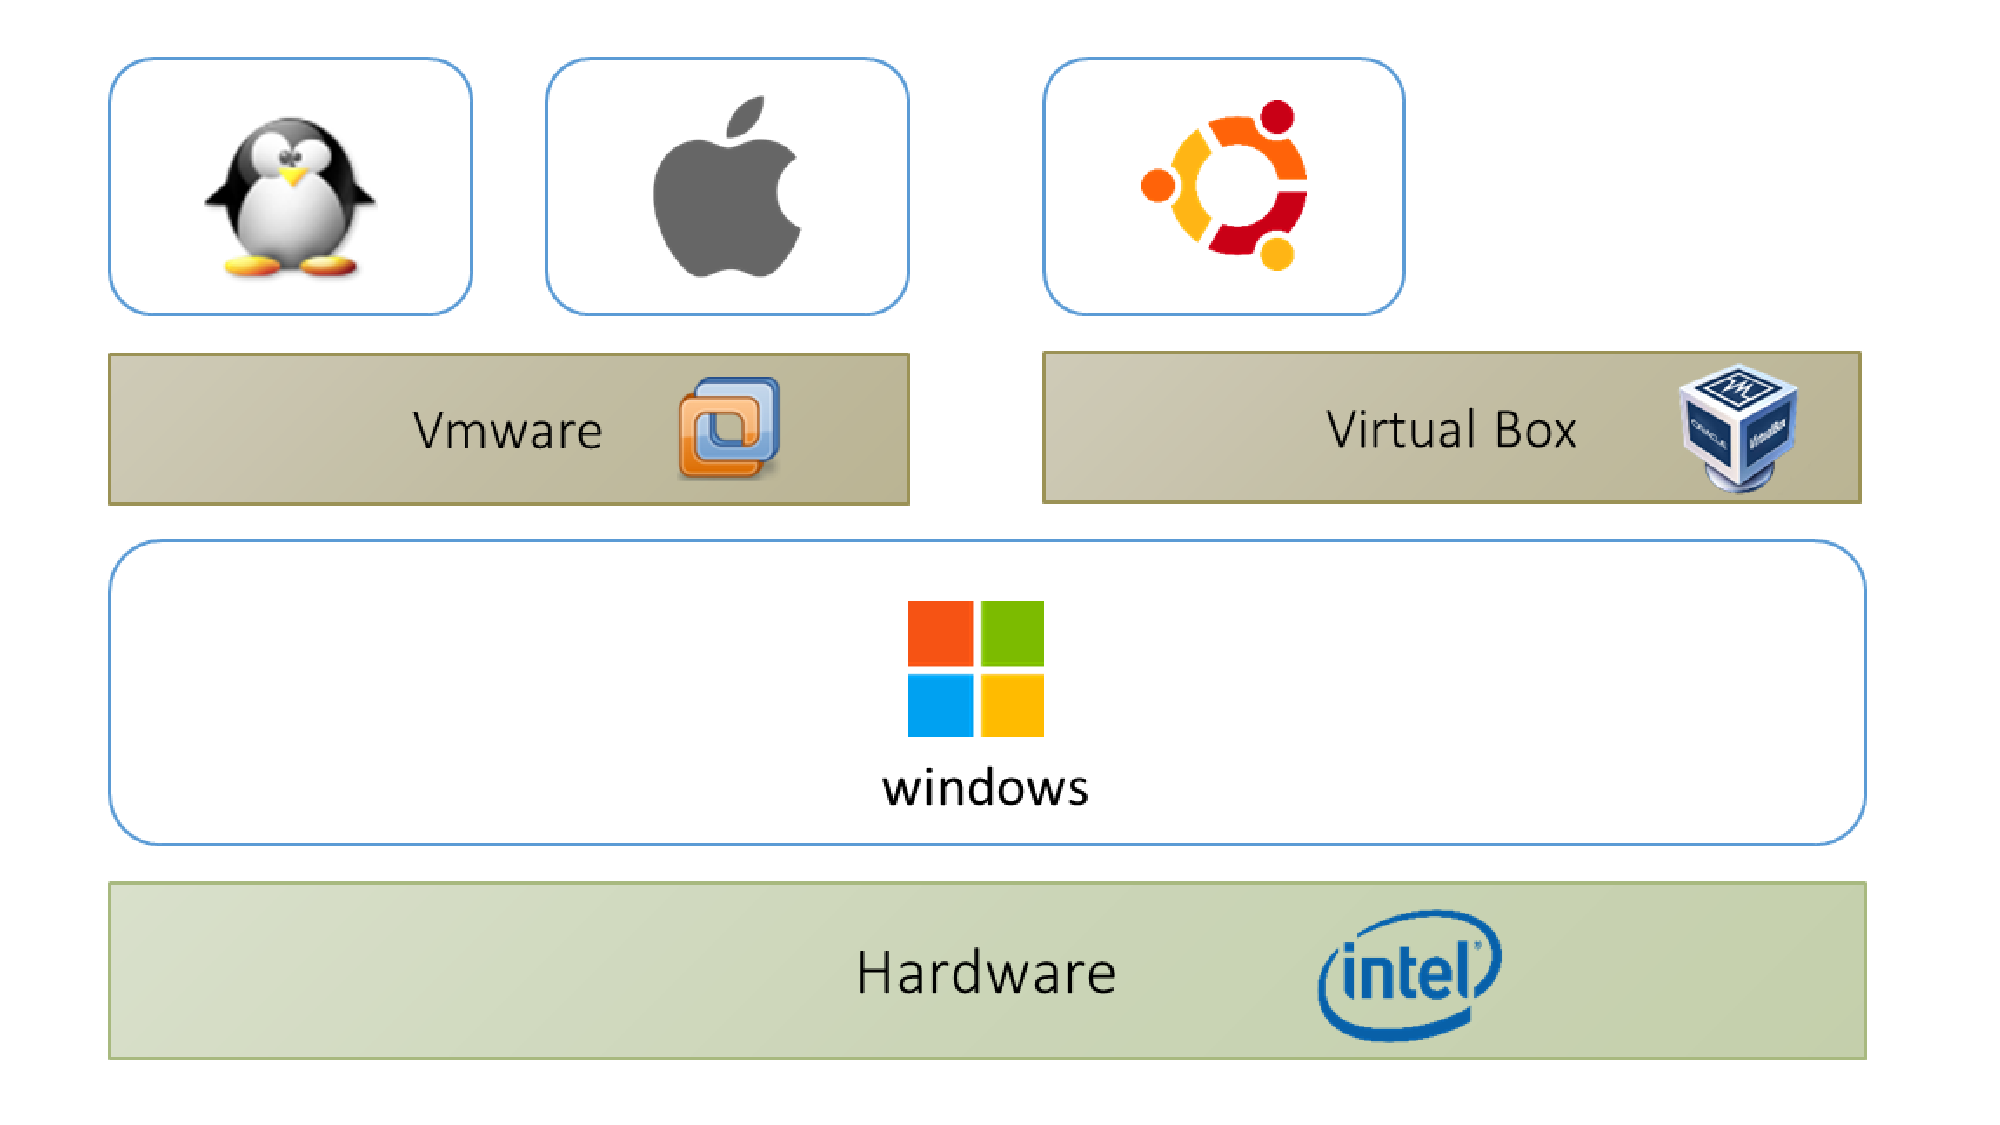
\includegraphics[scale=.4]{type2}
\caption{Type 2 hypervisor}
\label{fig:Type 2 hypervisor}
\end{figure}
\end{itemize}

\subsection{Xen Hypervisor}
Xen~\cite{Barham:2003:XAV:1165389.945462} is a widely known Type 1 hypervisor that allows the execution of virtual machines in guest domains~\cite{King_operatingsystem}. Figure~\ref{fig:Type 2 hypervisor} represents a diagram showing the different layers of a Type 1 hypervisor system. The hypervisor itself forms the lowest layer, which consists of the hypervisor kernel and the virtual machine monitors. The kernel has direct access to the hardware and is responsible for resource allocation, resource scheduling and resource sharing. A hypervisor is a layer responsible for virtualizing and providing resources to a given operating system.
\\[3mm]
The purpose of a hypervisor is to allow guest operating systems to be run. Xen runs guest operating systems in environments known as domains. \texttt{Domain 0} is the first guest to run, and has elevated privileges. Xen loads a \texttt{domain 0} guest kernel during boot. Other unprivileged domains are called \texttt{domain U}. The Xen hypervisor does not include device drivers. Device management is included in privileged \texttt{domain 0}. \texttt{Domain 0} uses the device drivers present in the guest operating system. However, \texttt{domain U} accesses devices using a split device driver architecture. In the split device driver architecture a frontend driver in a guest domain communicates with a backend driver in \texttt{domain 0}.
\\[3mm]
Figure~\ref{xen-split2} shows how an application running in a \texttt{domain U} guest writes data on the physical device. First, it travels through the file system as it would normally. However, at the end of the stack the normal block device driver does not exist. Instead, a simple piece of code called the frontend puts the data into the shared memory. The other half of the split device driver called the backend, running in the \texttt{domain 0} guest, reads the data from the buffer and sends it way down to the real device driver. The data is written on the actual physical device. In conclusion, split device driver can be explained as a way to move data from the \texttt{domain U} guests to the \texttt{domain 0} guest, usually using ring buffers in shared memory~\cite{Chisnall:2007:DGX:1407351}.
\begin{figure}[!h]
\centering
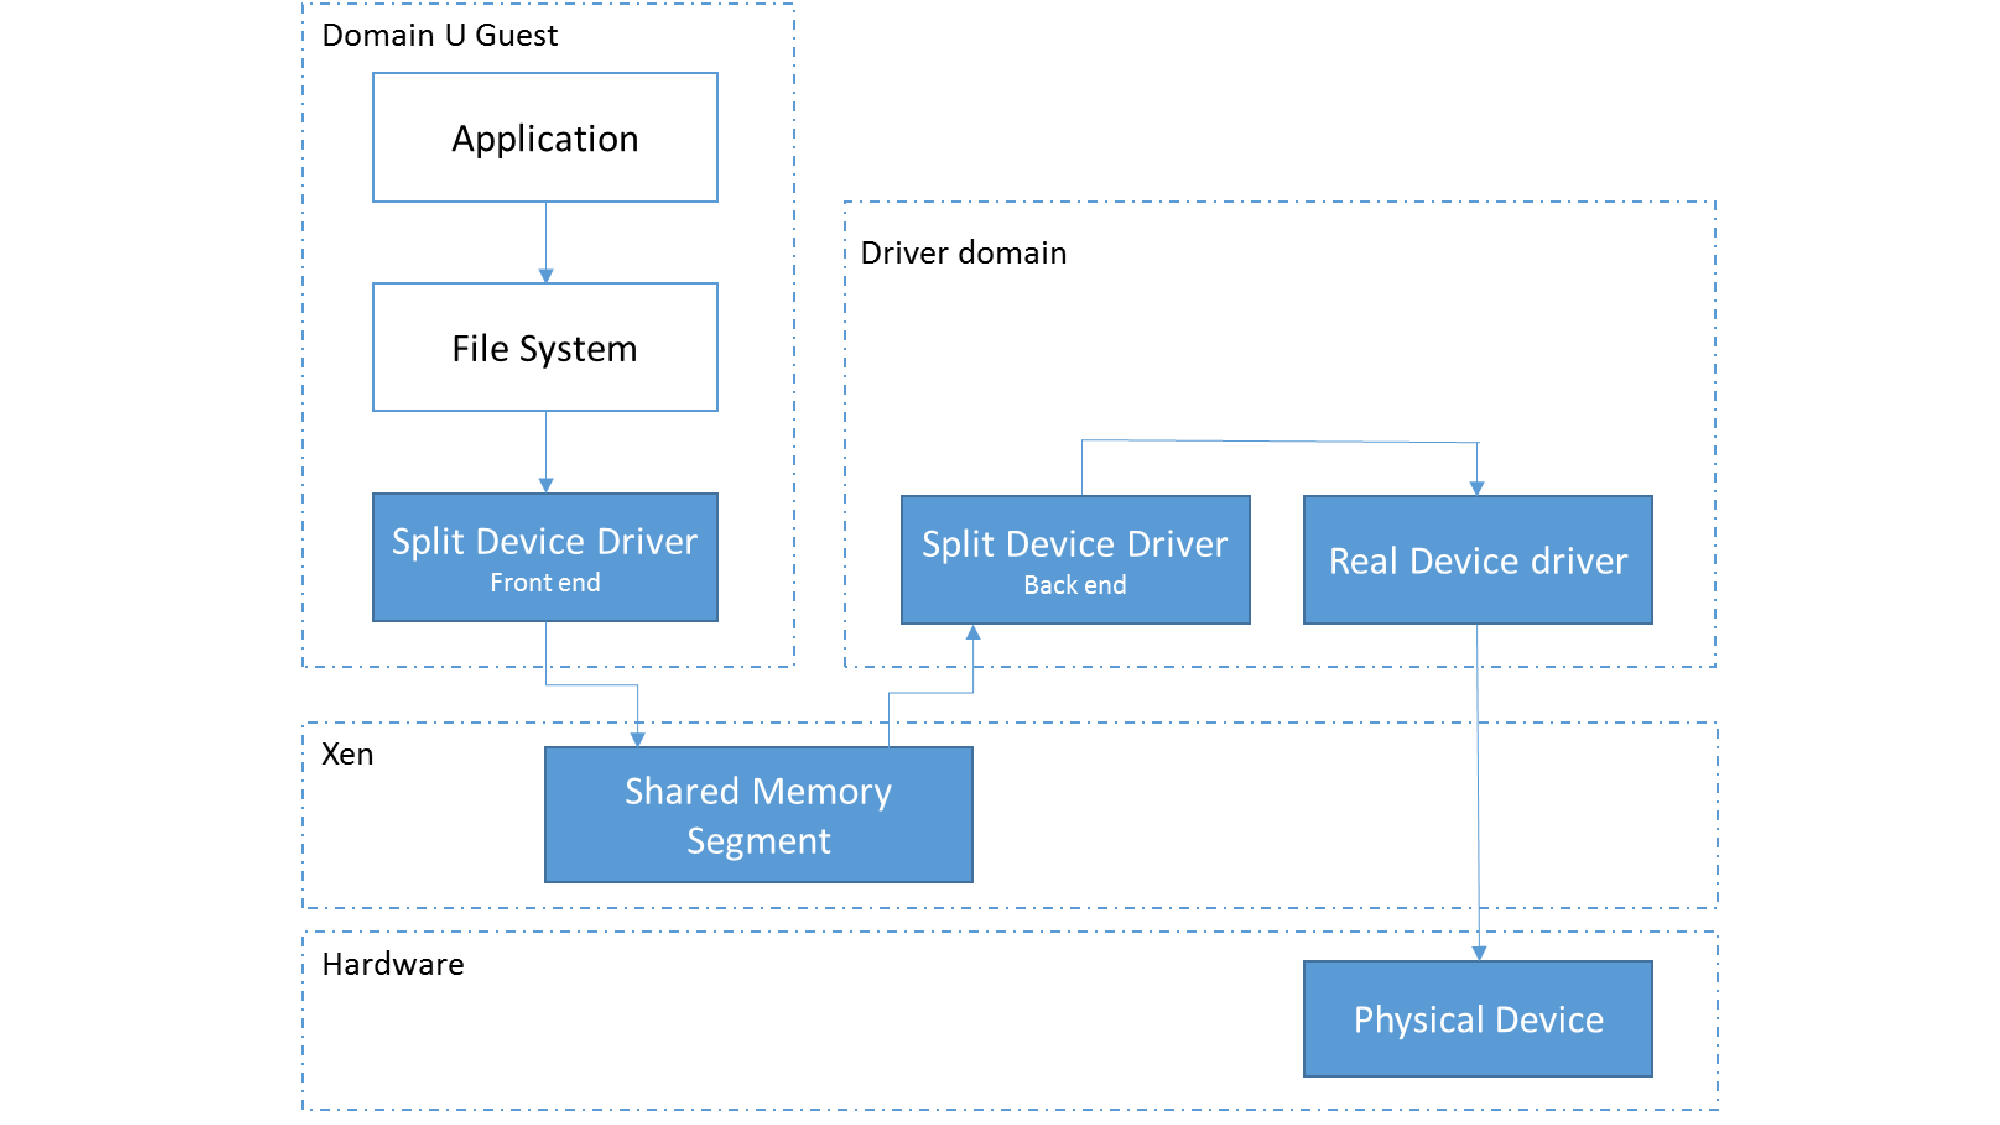
\includegraphics[scale=.50]{xen-split-fs}
\caption{Xen split device driver}
\label{xen-split2}
\end{figure}
\\[3mm]
Xen provides an inter-domain memory sharing API accessed through the guest kernel extensions and an interrupt-based inter-domain signaling facility called event channels to implement the efficient inter-domain communication. Split drivers use memory sharing APIs to implement I/O device ring buffers to exchange data across domains.
\begin{figure}[!h]
\centering
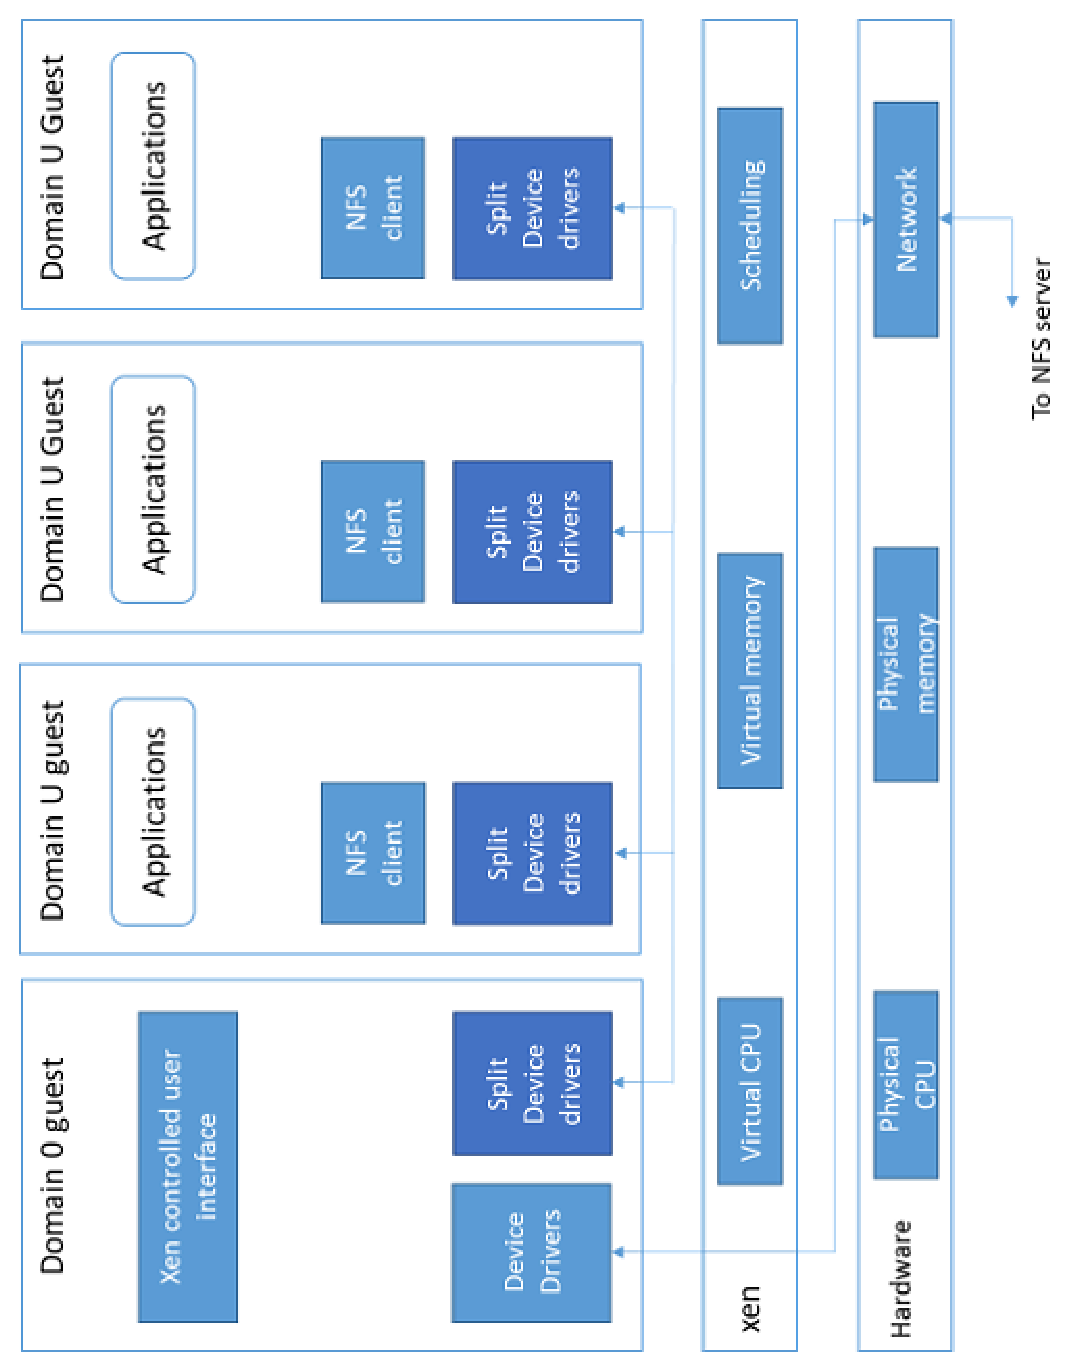
\includegraphics[scale=.50]{xen}
\caption{Xen}
\label{xen}
\end{figure}
\\[3mm]
In Xen's isolated driver domain implementation, Xen uses shared I/O ring buffers and event channel~\cite{Barham:2003:XAV:1165389.945462, Nikolaev:2013:VOS:2517349.2522719, Ruslan}.

\subsubsection*{Hypercalls and Events}
Hypercalls and event channels are the two mechanisms that exist for interactions between the Xen hypervisor and domains. A hypercall is a software trap from a domain to the Xen hypervisor, just as a syscall is a software trap from an application to the kernel~\cite{hypercall}. Domains use the hypercalls to request privileged operations like updating pagetables. 
\\[3mm]
An event channel is to the Xen hypervisor as a hardware interrupt is to the operating system. An event channel is used for sending asynchronous notifications between domains. Event notifications are implemented by updating a bitmap. After scheduling pending events from an event queue, the event callback handler is called to take appropriate action. The callback handler is responsible for resetting the bitmap of pending events, and responding to the notifications in an appropriate manner. A domain may explicitly defer event handling by setting a Xen readable software flag: this is analogous to disabling interrupts on a real processor. Event notifications can be compared to traditional UNIX signals acting to flag a particular type of occurrence. For example, events are used to indicate that new data has been received over the network, or used to notify that the a virtual disk request has completed. 

\subsubsection*{Data Transfer: I/O Rings}
\label{subsec:io rings}
Hypervisor introduces an additional layer between guest OS and I/O devices. Xen provides a data transfer mechanism that allows data to move vertically through the system with minimum overhead. 
\begin{figure}[!ht]
\centering
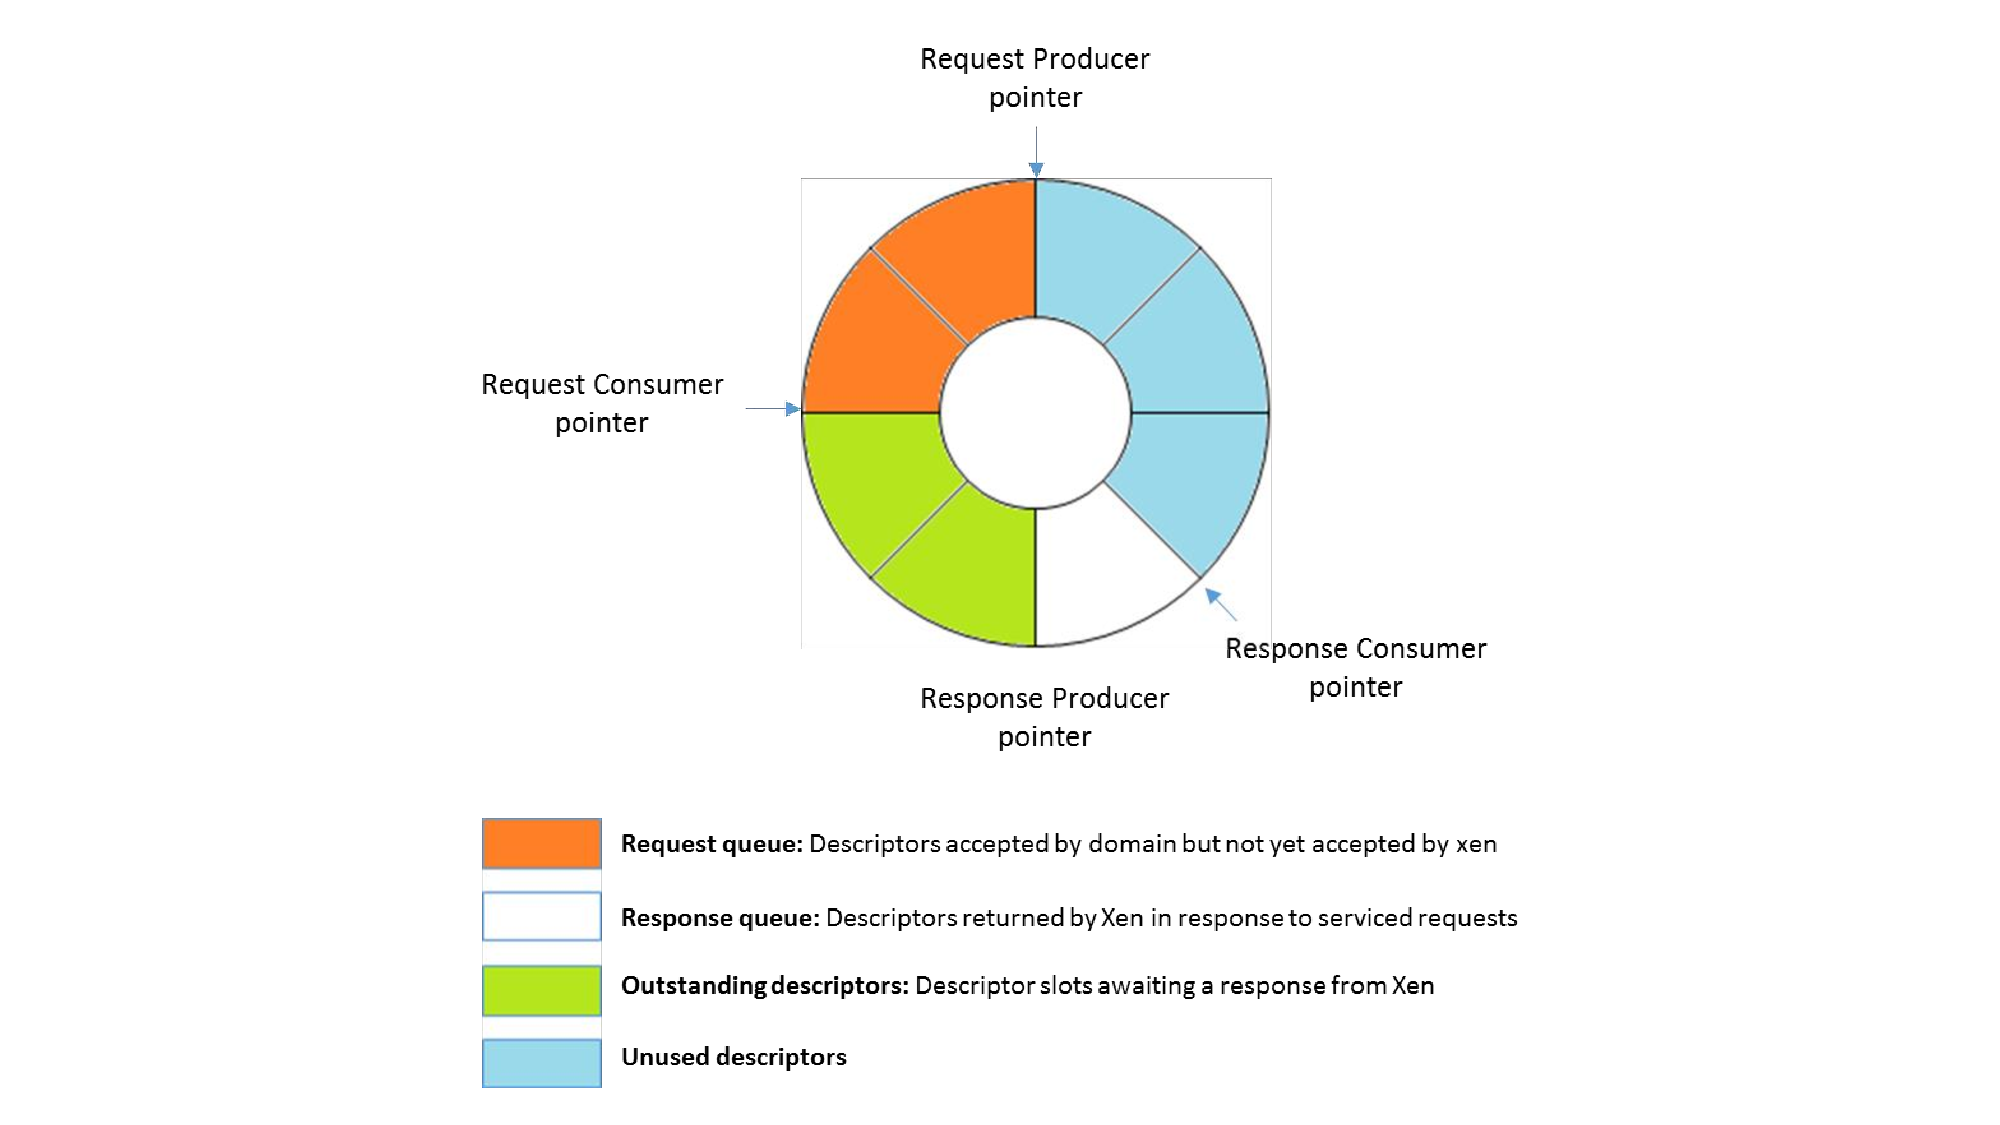
\includegraphics[scale=.5]{IObuffer}
\caption{Ring I/O buffer}
\label{fig:Ring buffer}
\end{figure}
\\[3mm]
Figure~\ref{fig:Ring buffer} shows the structure of an I/O descriptor ring. An I/O descriptor ring is a circular queue of descriptors allocated by a domain. These descriptors do not contain I/O data. However, I/O data buffers are allocated separately by the guest OS and is indirectly referenced by these I/O descriptors. Access to an I/O ring is based around two pairs of producer-consumer pointers.
\begin{enumerate}
\item Request producer pointer: A domain places requests on a ring by advancing a request producer pointer. 
\item Request consumer pointer: The Xen hypervisor removes requests pointed by a request producer pointer. These requests are removed by advancing a request consumer pointer.
\item Response producer pointer: The Xen hypervisor places responses on a ring by advancing a response producer pointer. 
\item Response consumer pointer: A domain removes responses pointed by a request producer pointer. These responses are removed by advancing a response consumer pointer.
\end{enumerate} 
The requests are not required to be processed in a specific order. I/O rings are generic to support different device paradigms. For example, a set of \texttt{requests} can provide buffers for read data of virtual disks; subsequent \texttt{responses} then signal the arrival of data into these buffers. 
\\[3mm]
The notification is not sent for production of each request and response. A domain can en-queue multiple requests and responses before notifying the other domain. This allows each domain to trade-off between latency and throughput.
\begin{figure}[!ht]
\centering
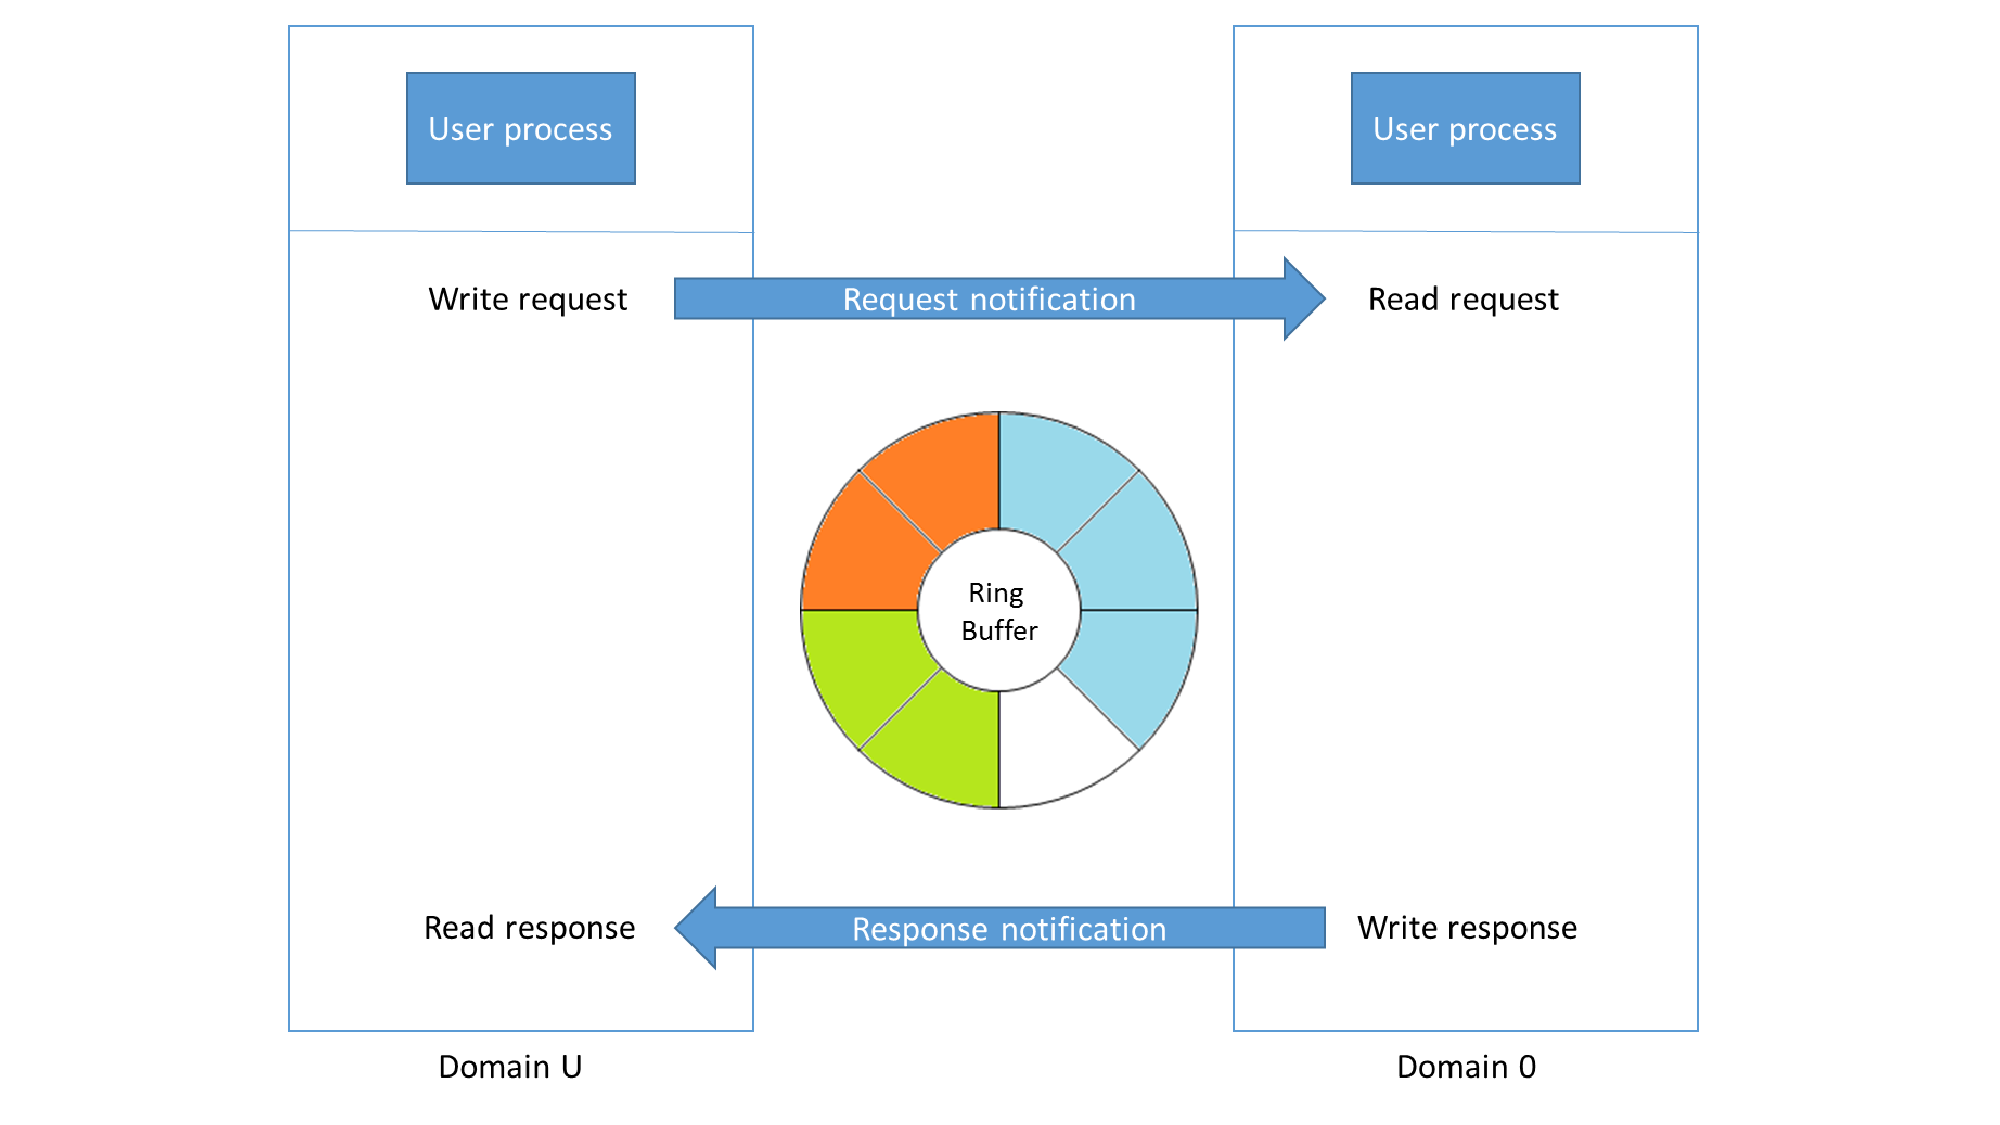
\includegraphics[scale=.5]{IObuffer2}
\caption{Ring I/O buffer}
\label{fig:Ring buffer}
\end{figure}

\subsection*{Shared Pages}
\label{subsec:sharedpages}
\subsubsection*{Grant Table} 
Grant tables are a mechanism provided by the Xen hypervisor for sharing and transferring frames between the domains. It is an interface for granting foreign access to machine frames and sharing memory between underprivileged domains provided by the Xen hypervisor. In Xen, each domain has a respective grant table data structure, which is shared with the Xen hypervisor. The grant table data structure is used by Xen to verify the access permission other domains have on the page allocated by a domain~\cite{granttable}.

\subsubsection*{Grant References}
Grant references are the entries in a grant table. A grant reference entry has every detail about the shared page. The Xen hypervisor virtualizes the physical memory, it is difficult to know the correct machine address of a frame for a domain. The biggest difficulty in sharing the memory between domains is knowing its correct machine address. A grant reference removes the dependency on the real machine address of the shared page. Hence, a grant entry makes it possible to share the memory between domains.\cite{Chisnall:2007:DGX:1407351, Barham:2003:XAV:945445.945462, granttable} 

\ifbool{toShowBibliography}{\bibliography{references}}{}
